% !TeX program = xelatex

\documentclass[final]{cubedoc}

\title{PCB Handbook}
\docid{AcubeSAT-OBC-G-009}
\author{Theodoros Katzalis}

\changelog{13/08/2019}{0.1}{INTERNALLY RELEASED}{Initial revision.}
\changelog{15/08/2019}{0.2}{INTERNALLY RELEASED}{Remove WIP from title and fix some typos.}
\changelog{14/08/2020}{0.3}{INTERNALLY RELEASED}{
	Updated:
	\begin{itemize}
		\item Rules of thumb.
		\item Identification of design and PCB design guidelines regarding high speed applications. The last one is referred as Design for Performance.
		\item Links are archived.
	\end{itemize}
	
	\bigskip
	
	Added: 
	\begin{itemize}
		\item References and image sources.
		\item Footnotes
		\item Design for Testing and Design for Manufacturing.
		\item An overview of simulation and analysis.
		\item Checklist
	\end{itemize}
	
	\bigskip
	
	Deleted:
	\begin{itemize}
		\item The Disclaimer section
	\end{itemize}
}

\usepackage{wrapfig}
\usepackage{subcaption}
\usepackage{hyperref}


\begin{document}
	
	\section{Preface}
	%What is the purpose of this report? How to read this report? What sections you can skip? If you are in x subsystem you might be find useful these y sections…
	%Learning materials are spread throughout the report, but if you want a synopsis you can found it in the end of this report! In “what is a PCB ?”, where the fabrication process is explained, it is focused on how professional manufacturers do their jobs and not how you can do it yourself. On the other hand, a DIY part would be very nice to have in the upcoming versions!Sometimes I was trying to use simple words for better comprehension just to feel what I was trying to say, so bare with me!!
	
	The purpose of this report is to make the reader feel familiar with the PCB fabrication  and to give an insight about the PCB guidelines when the time for design comes. So, it is divided in two main conceptual parts: \textbf{"What is a PCB?"} and \textbf{"How to design a PCB?"}. In the first part, we will make a short introduction about different types of PCBs, their materials and the overall structure. The second part isn't oriented on how to use a CAD tool, but highlights the potential problems in signal integrity and the countermeasures.
	
	%If you don't have time to read thoroughly the whole report, then you should check the the \autoref{subsec:techniques} (PCB Layout techniques) and \autoref{subsec:thumb} (Rules of thumb).
	%How I learned about PCB, where tou could find useful information + just design, print, DIY, play, do stuff!
	
	%\section{Disclaimer}
	%This report is marked as \textbf{W}ork \textbf{I}n \textbf{P}rogress, because a lot more should be added in order to have a well completed-organized-detailed guide for PCB design. Although, I think that the the word “complete” is very uncertain and undefined, but it means that a lot more things will be discovered throughout the PCB journey, so everyone can share their personal knowledge and experience. Also, due to time constraints, some topics aren’t described in-depth. It is worth mentioning that we won’t reinvent the wheel, but we are collecting information to provide an orientation/guidance to those who thrive to design a PCB. I hope that the current version is adequate to develop an insight about PCBs and the mindset for designing quite efficiently the AcubeSAT’s boards, in the time remaining. Of course, more questions and clarifications can be made individually with the AcubeSAT’s members that have some experience in PCB design. And...of course, for the time being, this report is for internal release. 
	
	\section{What is a PCB?}
	
	\begin{wrapfigure}{R}{0.4\textwidth}
		\centering
		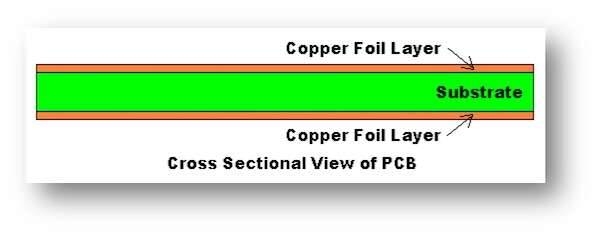
\includegraphics[width=0.4\textwidth]{assets/simple_2_layer_PCB.jpg}
		\caption{2-layer PCB \small{(\href{https://web.archive.org/web/20200813141542/https://www.edn.com/pcb-design-basics/}{image source})}}
		\label{fig:1}
	\end{wrapfigure}
	
	PCB is a \textbf{P}rinted \textbf{C}ircuit \textbf{B}oard and is  a “sandwich” of conductive and non-conductive materials that cooperate to control the electrical flow between electrical components. It’s the place, where these components can be hosted and communicate with each other and can be described as their mechanical and electrical support. PCBs have developed a lot throughout the years: The irreversible progress of modern electronics changed radically the performance and the specifications along with the considerations and the new challenges that the whole industry must face. Things are getting smaller, faster, light weight and reliable. Just check the figure 2 and you will feel how time change things!
	
	
	
	\begin{figure}[h!]
		\centering
		\begin{subfigure}{.5\textwidth}
			\centering
			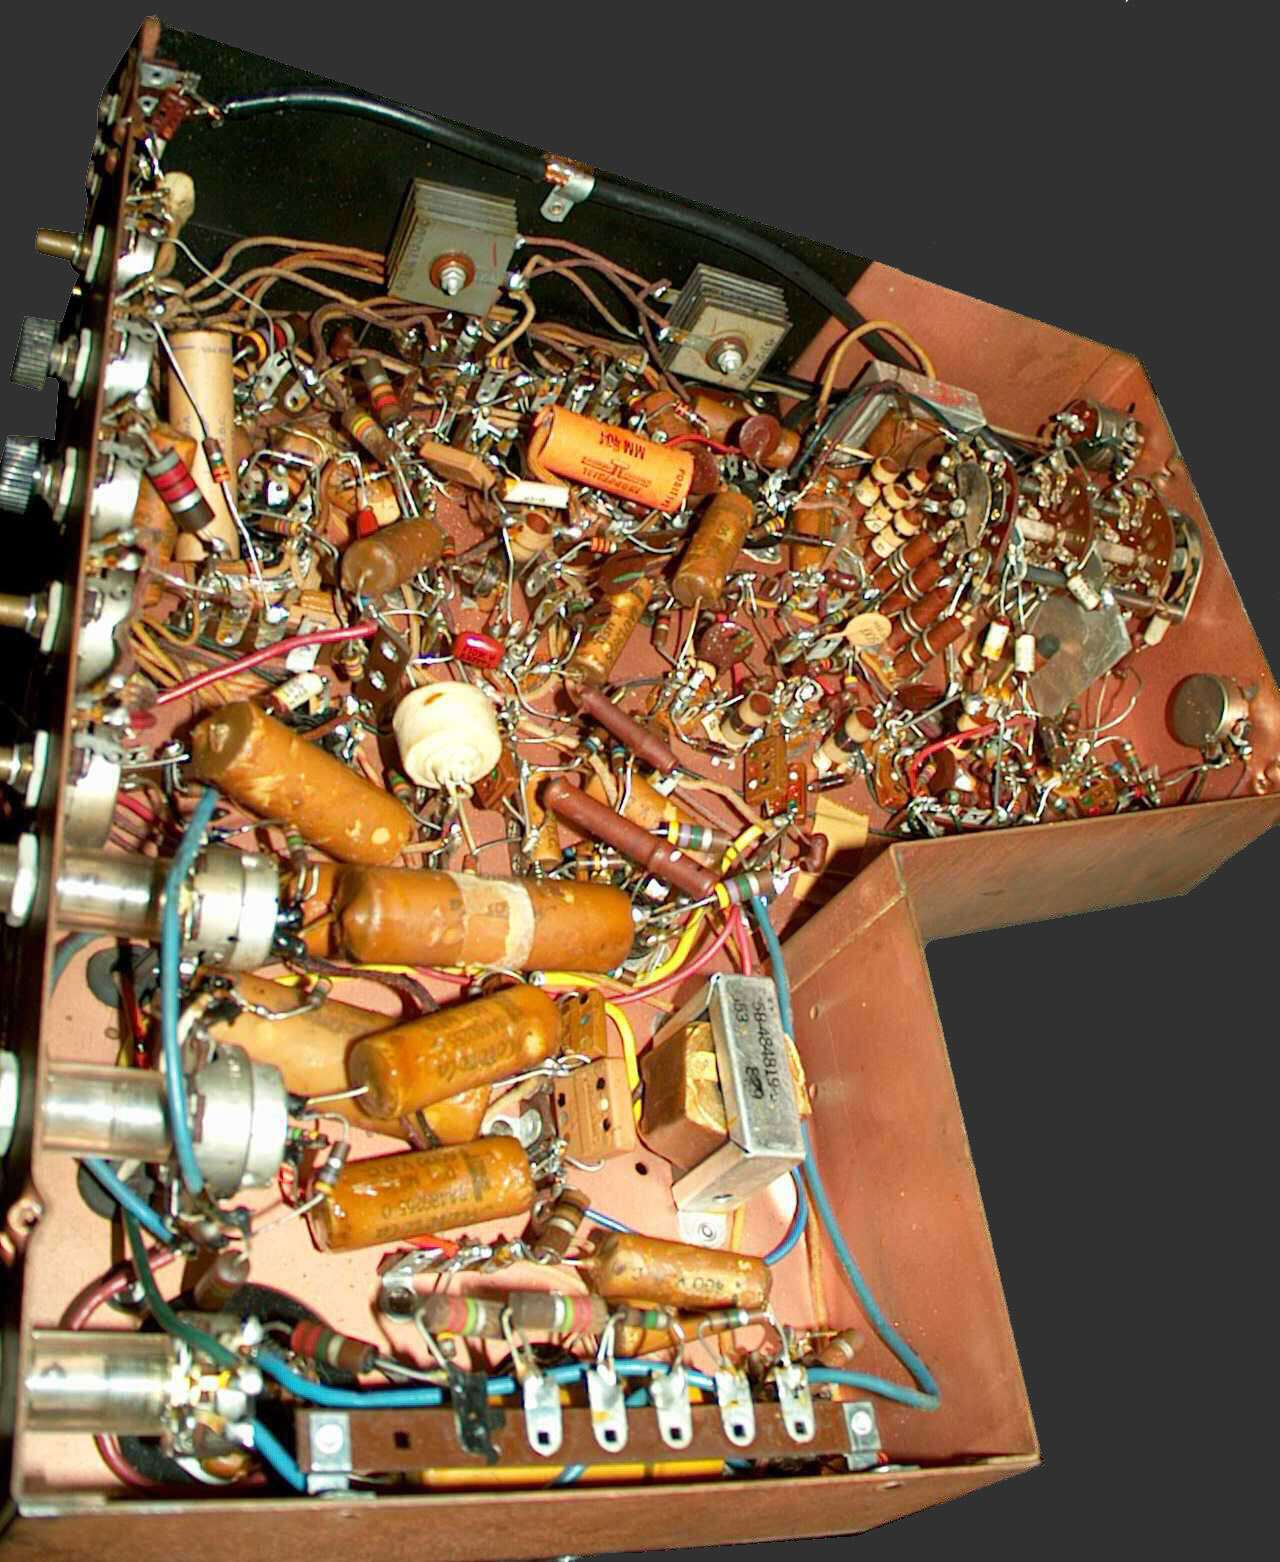
\includegraphics[height=0.25\textheight, width=.8\textwidth]{assets/old_school_TV_PCB.jpg}
			\caption{\href{https://web.archive.org/web/20200813142459/https://www.edn.com/the-pcb-is-the-most-important-component-of-your-design/}{image source}}
			\label{fig:sub1}
		\end{subfigure}%
		\begin{subfigure}{.5\textwidth}
			\centering
			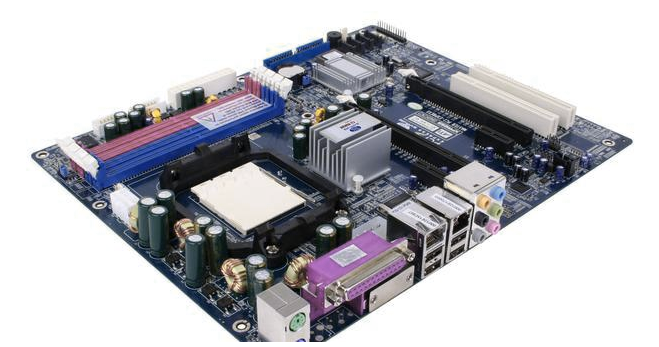
\includegraphics[height=0.25\textheight, width=.8\textwidth]{assets/modern_pcb.png}
			\caption{\href{https://web.archive.org/web/20200813143650/https://www.pcbsky.com/computers.html}{image source}}
			\label{fig:sub2}
		\end{subfigure}
		\caption{An old school TV's PCB on the left and a modern PCB on the right}
		\label{fig:test}
	\end{figure}
	
	\subsection{Materials}
	
	As mentioned earlier, PCB is mainly a stack of conductive and non-conductive materials:
	
	\begin{itemize}
		\item Conductive: \textbf{Copper foils}
		\item Non-conductive: Dielectric substrate (the base that hold the PCB together and separate the copper foils) like \textbf{FR-4}. The choice of the substrate is a function of thermal and electrical performance. For example, ceramic substrates is preferred in demanding thermal applications due to the higher thermal conductivity.
	\end{itemize}
	
	To be more precise, FR4 laminate coated with copper is called copper clad laminate (CCL). The copper foil is glued in high temperatures with the pre-preg (pre-impregnated) that is fiberglass with impregnated epoxy resin (uncured FR4). Thus CCL is the fundamental block of a PCB (\href{https://www.pcbway.com/blog/PCB_Basic_Information/Copper_Clad_Laminate.html}{source}).
	
	\begin{figure}[h]
		\centering
		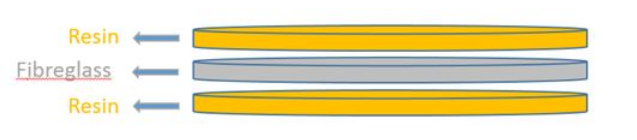
\includegraphics[width=0.8\textwidth,height=0.8\textheight,keepaspectratio]{assets/fiberglass_resin.png}
		\caption{Prepreg, uncured FR-4 \small({\href{https://www.pcbway.com/blog/PCB_Basic_Information/Copper_Clad_Laminate.html}{image source}})}
	\end{figure}
	
	Are PCBs consisted only of copper and substrate? Actually, no! In PCB fabrication, more complementary processes are required (subsection \ref{subsec:complementary}).
	
	But, first of all let’s visualize and comprehend the structure and the manufacturing process of these magic boards! PCBs can have different numbers of layers and sides, but can also come in changing inflexibilities. 
	
	\subsection{Inflexibility}
	In terms of inflexibility, there are three main types: 1) rigid, 2) flex and 3) rigid-flex PCBs:
	
	\subsubsection{Rigid}
	The first thing that is coming to your mind when thinking a PCB is probably the rigid one. A motherboard is a characteristic example. Basically, these type of boards  use a solid substrate material that prevents the board from changing its shape. 
	
	\subsubsection{Flex}
	As the name implies the advantage of the flex boards is the ability to flex! When there are tight mechanical constraints and little space, this type of boards are usually preferred. They can be either used as connectors reducing significantly the bulky size of typical connectors or as a fully assembled board. Common flex-materials to utilize these features are plastic like polyimide and polyester (\href{https://www.altium.com/rigid-flex-circuits-resources/flex-circuit-materials}{source}). Of course all of this comes with an extra cost than the rigid one.
	
	\subsubsection{Rigid-Flex}
	Rigid flex boards merge technology from both flexible and rigid circuit boards and they are consisted of flexible and rigid materials. A typical example could be two rigid boards connected with a flex one.
	
	%source for these kind of stuff are info provided by manufacturers and asselby houses, blogs.
	
	\begin{figure}[h!]
		\centering
		\begin{subfigure}{.3\textwidth}
			\centering
			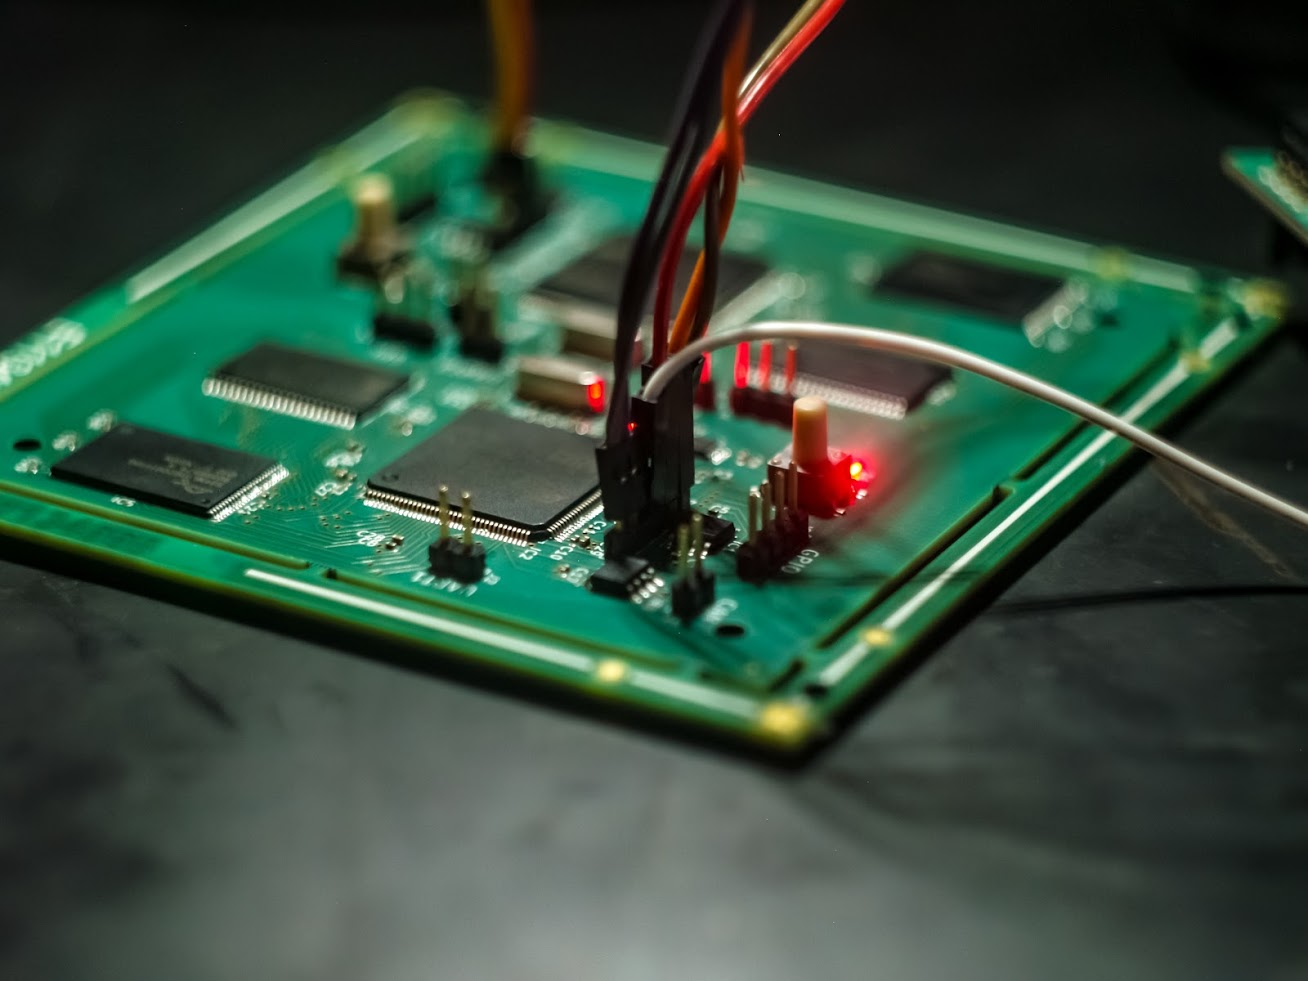
\includegraphics[height=0.2\textheight, width=.8\textwidth]{assets/rigid_obc.jpg}
			\caption{OBDH EM}
			\label{fig:sub1}
		\end{subfigure}%
		\begin{subfigure}{.3\textwidth}
			\centering
			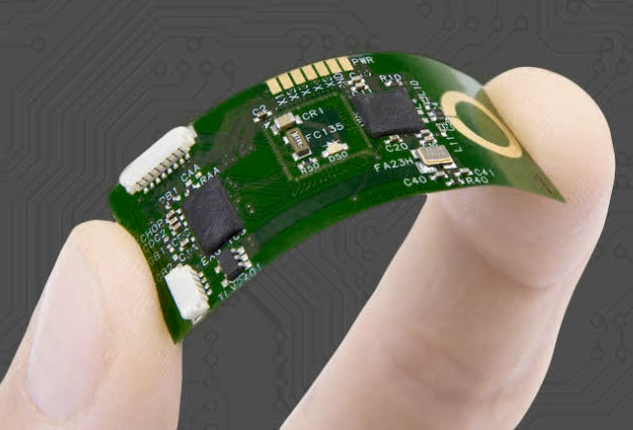
\includegraphics[height=0.2\textheight, width=.8\textwidth]{assets/flex.jpg}
			\caption{\href{https://web.archive.org/web/20200813150519/https://sfxpcb.com/flex-pcb-vs-ceramic-pcb/}{image source}}
			\label{fig:sub2}
		\end{subfigure}
		\begin{subfigure}{.3\textwidth}
			\centering
			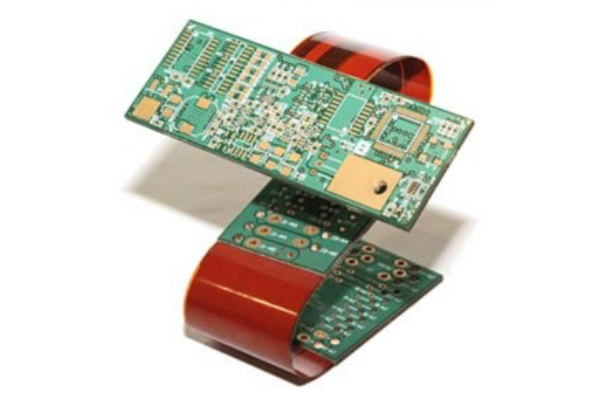
\includegraphics[height=0.2\textheight, width=.8\textwidth]{assets/rigid_flex.jpg}
			\caption{\href{https://web.archive.org/web/20200813145720/https://www.allaboutcircuits.com/technical-articles/pcbs-rigid-vs.-flexible-which-one-is-best-for-your-next-project/}{image source}}
			\label{fig:sub2}
		\end{subfigure}
		\caption{Rigid, flex and rigid-flex PCBs}
		\label{fig:test}
	\end{figure}
	
	%If you have been a little bit confused about PCBs…don’t worry! Keep reading and I hope that the following examples will help to make  the situation clear!
	From now on, we will be focused on simple and common rigid PCBs.
	
	\subsection{Layers}
	
	Printed Circuit Boards can be divided into layers. The increasing technological demands result to multi-layer boards and the stack up (the arrangement of copper layers and insulating layers)  is a very important factor. The number of layers range typically from 1 to 16 %(\href{https://en.wikipedia.org/wiki/List_of_integrated_circuit_packaging_types}{some} claim that 100-layer PCB is even possible to fabricate!)
	and usually, in the industry, even numbers are used. Using the term layers we are basically referring to the number of copper layers.
	
	\subsubsection{2-Layer}
	
	%\begin{figure}[h!]
	%    \centering
	%    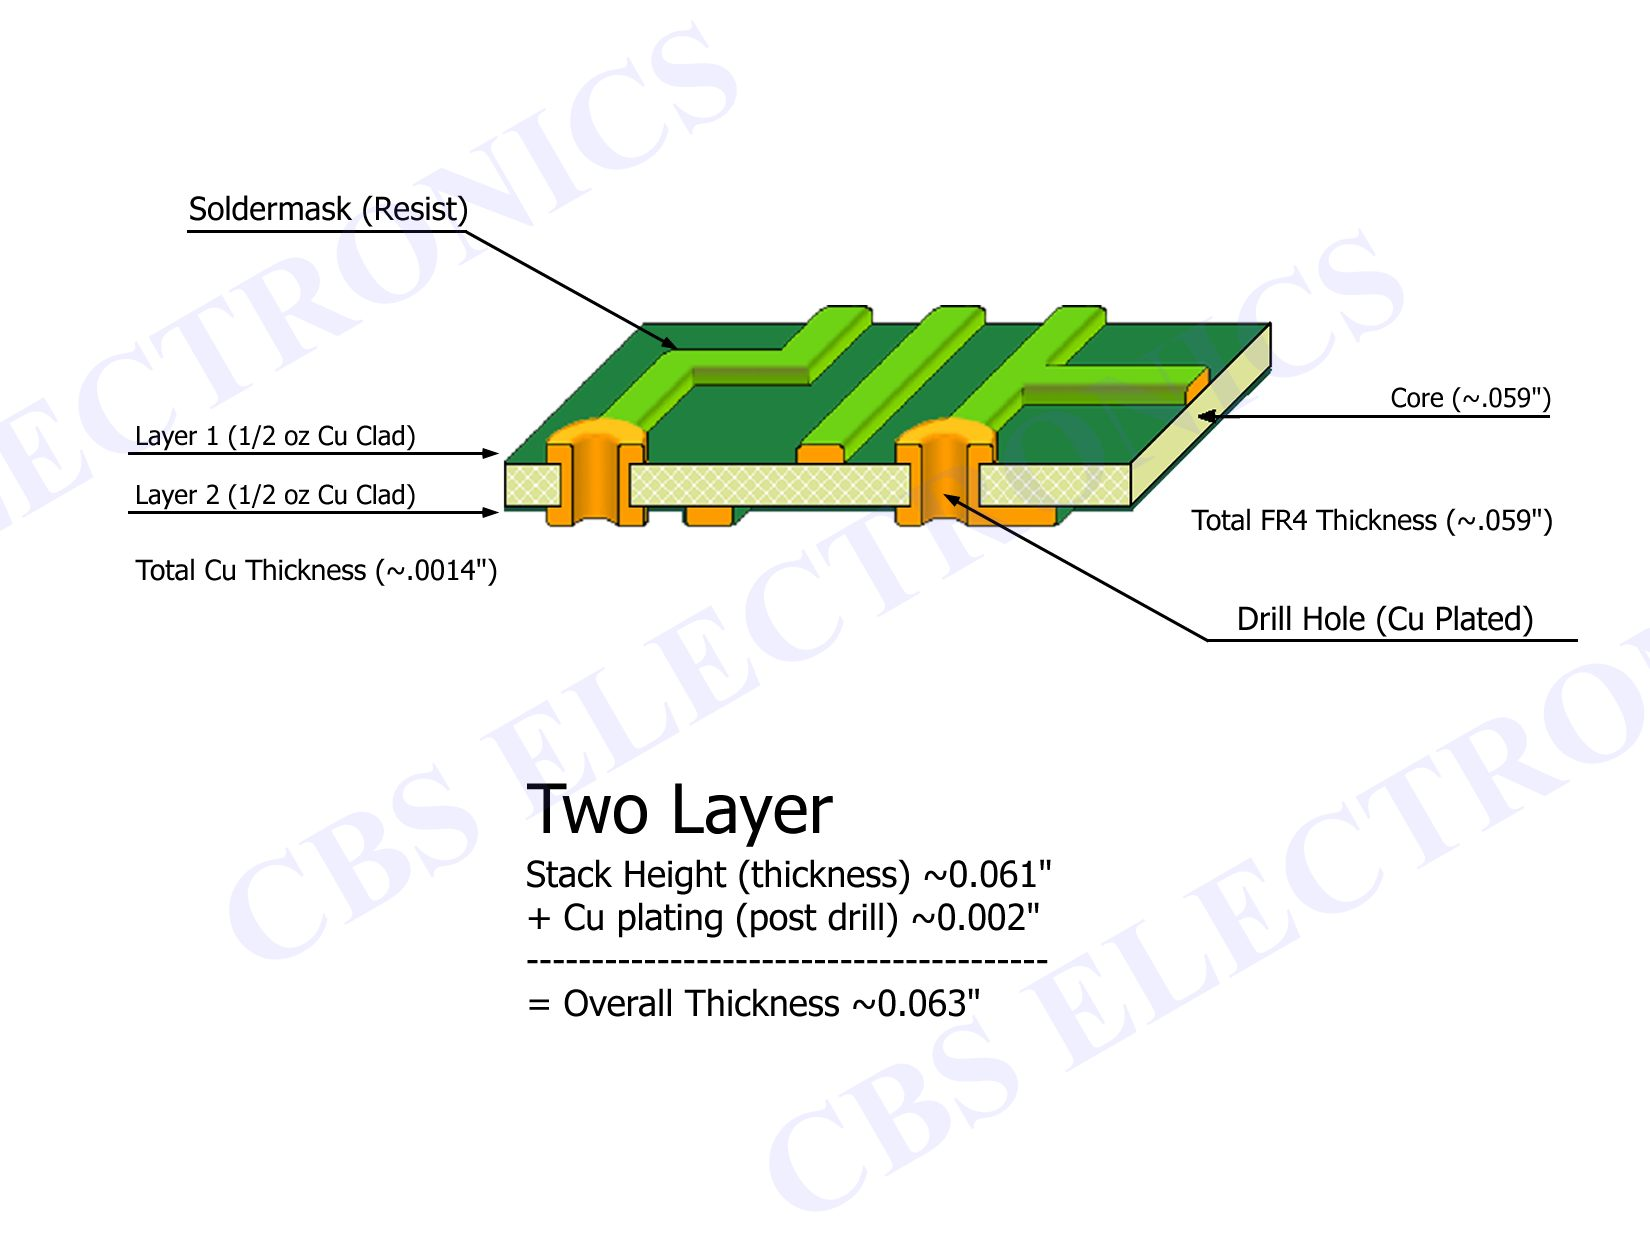
\includegraphics[height=0.45\textheight, width=\textwidth]{assets/2lyr_stackup.jpg}
	%    \caption{}
	%    \label{fig:my_label}
	%\end{figure}
	\begin{wrapfigure}{R}{0.3\textwidth}
		\centering
		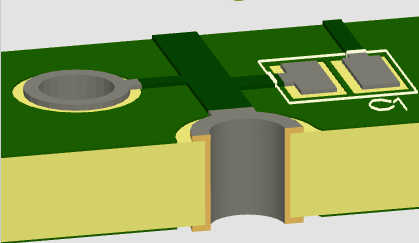
\includegraphics[height=.1\textheight, width=0.3\textwidth]{assets/2_layer_euro_3D.png}
		\caption{2-layer PCB, \small{source: Eurocircuits buildup feature}}
	\end{wrapfigure}
	
	A 2-layer board can be described as a copper clad laminate as we mentioned earlier. On these copper sides, the routing takes place. These copper paths called traces serve as the channel for the electrical components to interact with each other. In other words, the point of the copper is to carry electrical signals to and from the PCB, much like your nervous system carries signals between your brain and your muscles. 
	
	Now, you may be wondered, how it is possible traces that belong to different copper layers to be connected with each other? The answer is via (vertical interconnection access) and it is applied also to multi-layers. In short, they are holes plated with copper.
	
	\begin{figure}[h!]
		\centering
		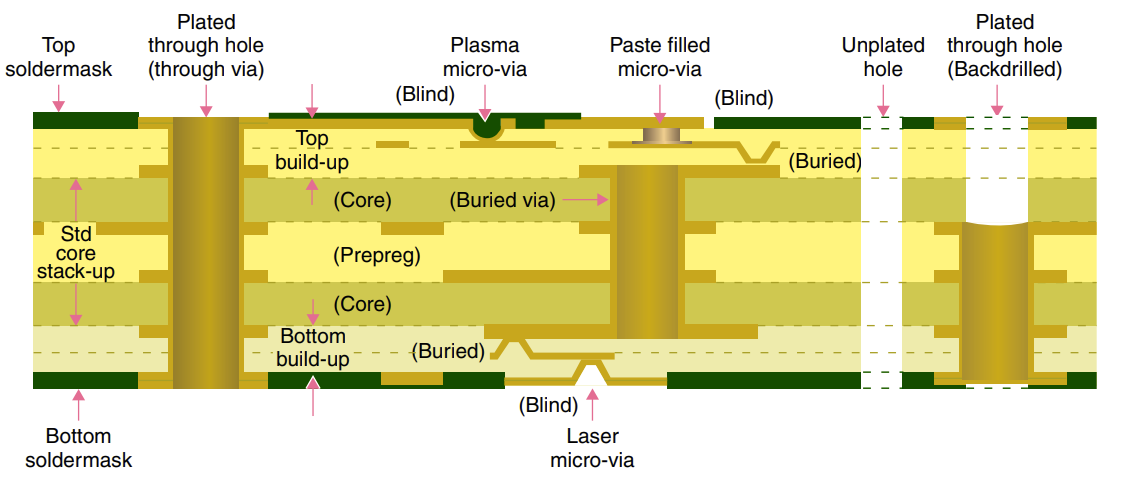
\includegraphics[width=\textwidth, height=.25\textheight]{assets/via.png}
		\caption{Different types of via for a multi-layer board, source the OrCAD book}
	\end{figure}
	
	About the core, it is a non-conductive substrate usually made of FR4. FR4 is used because it provides a solid, strong core and the most cost effective solution regarding dielectric strength, losses and heat dissipation. There are many types of FR4 though. Eventually, think of the substrate as the PCB’s “skeleton”. 
	%\href{https://www.twistedtraces.com/blog/fr4-printed-circuit-boards}{source}
	
	\subsubsection{4-Layer}
	Now, that we have a basic understanding about a 2-layer PCB, let’s jump to a 4-layer one:
	
	\begin{figure}[h!]
		\centering
		\begin{subfigure}{.4\textwidth}
			\centering
			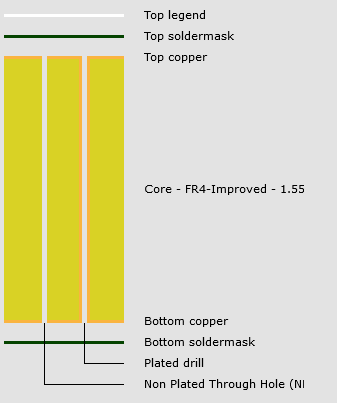
\includegraphics[height=0.25\textheight, width=\textwidth]{assets/2_layer_euro.png}
			\caption{source: Eurocircuits buildup feature}
		\end{subfigure}
		\begin{subfigure}{.4\textwidth}
			\centering
			\includegraphics[height=0.25\textheight, width=\textwidth]{assets/4_layer_PCB.png}
			\caption{\href{https://web.archive.org/web/20200813153211/https://docs.toradex.com/102492-layout-design-guide.pdf}{image source}}
		\end{subfigure}
		\caption{Typical stack-up dimensions fro a 2 (left) and 4 (right) layers boards}
	\end{figure}
	
	The multi-layer layers are basically a set of 2-layer boards glued together and this is also the main reason why even numbers are used. Furthermore, lamination is the process by which the core(s) of a printed circuit board are melted together through heat and pressure with copper layers and prepreg layers (in multi-layer PCBs). In other words, it is the process that creates a “sandwich” or multiple “sandwiches” connected together. It requires specific heating and pressure for specific periods of time based on materials used to ensure the PCB is made properly.  These laminates and the copper thickness comes in different sizes, too.
	
	% what is lamination is straight forward regarding resources
	
	\begin{figure}[h!]
		\centering
		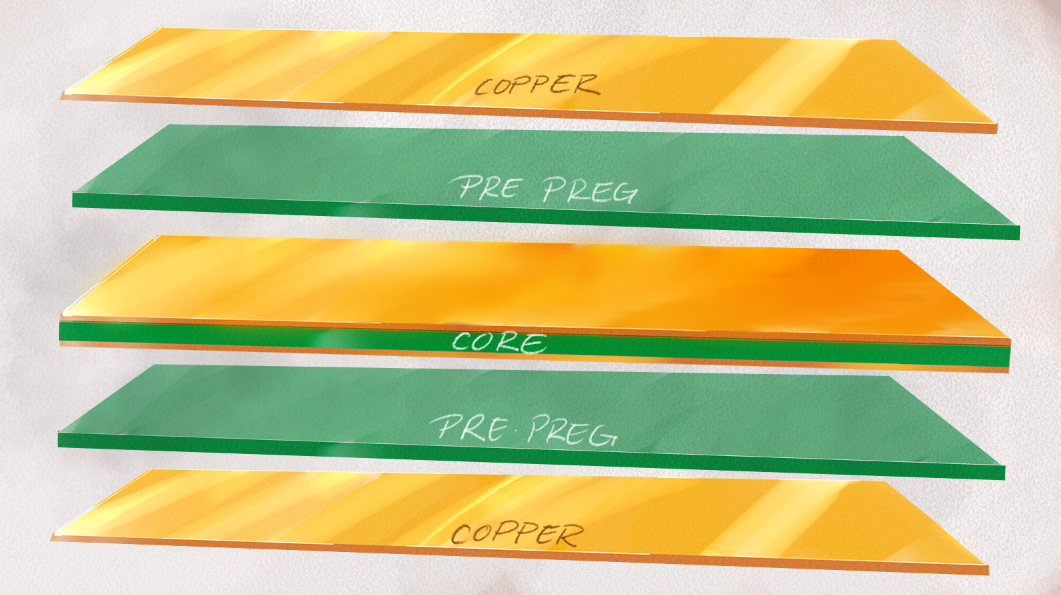
\includegraphics[height=.25\textheight]{assets/multi-layer-lamination.png}
		\caption{}
		\label{fig:my_label}
	\end{figure}
	
	Noticeable differences between the figure 7a and figure 7b are: 1) the height is approximately the same to these boards (0.063 inches = 1.6 mm) and 2) the \textbf{prepreg}. Someone could say, how it is possible for the overall thickness to be the same in 2 and 4 layers PCB? It’s because laminates and copper foils of different thickness are used to prevent increasing the height of it as the layers are increasing. So a 4-layer board is actually a set of two 2-layer boards separated by  the core, but the overall thickness is the same with a 2-layer design, because in the 4 layer-design the pairs have smaller thickness. A rule of thumb is to have the same thickness above and below of the core! (multi-layers boards can be mirrored).
	
	As we have stated, prepreg is a fiberglass impregnated with resin (FR4). The resin isn'
	t hardened yet so it can be used to glue the required copper foils. It is different with the core in the way that there is still the modular feature of curing, of bonding things together. The core is already cured with copper foils in both sides (copper clad laminate). Although there might be some differences in the materials and the electric, thermal properties between these two.
	%\href{https://resources.altium.com/p/pcb-core-vs-prepreg-material-what-designers-need-to-know}{source}
	
	\subsection{Complementary layers}
	\label{subsec:complementary}
	
	Except the fundamental copper layers and the substrate, there are some complementary processes during manufacturing that can be defined as extra layers (note: the term layers is used quite a lot and can have several meanings) and they are very useful and necessary nowadays. These are the soldermask, the surface finish/treatment, the silkscreen and the conformal coating. We are go intro great depth for the materials and their properties though.
	
	\begin{figure}[h!]
		\centering
		\centering
		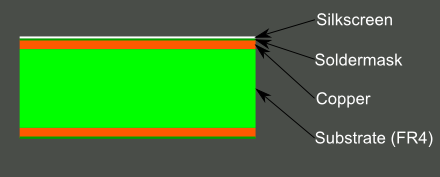
\includegraphics[keepaspectratio, height=0.25\textheight, width=.6\textwidth]{assets/2_layer_plus_silkscreen.png}
		\caption{\href{https://learn.sparkfun.com/tutorials/using-eagle-board-layout/all}{Image source}}
	\end{figure}
	
	
	
	\subsubsection{Soldermask}
	
	If you encountered a PCB, then the first thing that you would notice is the green color. This is called soldermask and is a thin polymer applied to the top and the bottom of a PCB. Overall the soldemask assists the functionality and durability of the board by protecting it from oxidation, corrosion, moisture and dust. It is used also for preventing manufacturing defects like solder bridges.  There are two basic categories of soldermask materials: liquid screen printed and photoimageable masks. Most of the times the soldermask choice in special applications like aerospace will be dictated by standards. It is worth mentioning that the green color is the most distinctive but of course it can have other colors too. There are a few reasons why the green is the most common one like better visual inspection.
	
	% source for color, \href{http://www.seeedstudio.com/blog/2017/07/23/why-are-printed-circuit-boards-are-usually-green-in-colour/}{this}
	
	% \href{https://resources.altium.com/p/how-choose-correct-solder-mask-your-pcb}{altium source}
	
	%source for the soldermask the OrCAD book
	
	\subsubsection{Surface finish}
	
	
	A PCB surface finish is a coating applied above the pads, the exposed copper areas. It is applied for two basic reasons: to ensure solderability and to protect exposed copper circuitry. As there are many types of surface finishes, selecting the right one is no easy task, especially as SMDs have become more complex and regulations such as RoHS and WEEE have changed industry standards.
	
	There are many types of surfaces. Namely we have: Hot air solder leveling (HASL), Immersion Tin (ImSn) or Silver (ImAg), Electroless Nickel Imerssion Gold (ENIG) and Electroless Nickel Electroless Palladium Immersion Gold (ENEPIG), Organic Solderability Preservative (OSP). The most popular in the old days was HASL.
	% source about the old one, \href{http://blog.optimumdesign.com/pcb-surface-finishes-comparison-hasl-osp-enig}{this}
	Each one of those has of course its advantages and its disadvantages. The most common one probably is the ENIG.
	
	% \href{https://www.pcbcart.com/article/content/surface-finish-intro-and-comparision.html}{source}
	
	\begin{figure}[h!]
		\centering
		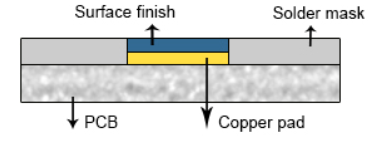
\includegraphics[keepaspectratio, height=0.2\textheight, width=.6\textwidth]{assets/surface_finish.png}
		\caption{\href{https://www.pcbcart.com/article/content/surface-finish-intro-and-comparision.html}{image source}}
	\end{figure}
	
	\subsubsection{Silkscreen}
	
	Silkscreen has no electrical purpose and is usually white and human readable letters, normally used to identify components, test points, PCB part numbers, warning symbols, company logos, date codes and manufacturer marks. This, in turn, makes it easier for electronics assemblers to place each PCB in the proper place and in the right direction on each component. It gives a more artistic tone in the PCB, too!
	
	%(maybe I can put the silkscreen layer of the OBC PCB)
	
	\subsection{Assembly}
	
	After the design and the bare board fabrication have finished, the time for soldering\footnote{Soldering is used both to attach components physically to the PCB and to provide electrical conductivity between the component’s leads and the PCB traces. The most common one is the Sn63/Pb37.} and component placement has come (populated board). The process that is responsible for this is called assembly and the board with the combined components is called PCBA (Printed Circuit Board Assembly).
	
	PCBs can be assembled \textbf{manually} or by \textbf{automatic} machinery. Manually assembled is related with placing and soldering the components by hand. This is suitable for prototypes and low volume production. A mixed process with hand placement and automatic soldering can also be used as a strategy regarding the manual method. For the automated assembly, pick and place machines are substituting the hands of the assemblers and the soldering process can be divided to reflow and wave soldering. 
	
	The first one is used for SMDs and the second one mostly for through hole or for a mixed set up with both package types. 
	As the high speed applications are increasing, SMT is replacing the through-hole due to better electrical performance (inductance and capacitance of the leads) and size costraints. Thus the wave soldering is used less except some special applications (e.g. power devices).
	
	\subsubsection{Conformal coating}
	
	Very briefly, conformal coating is an additional step of the assembly process. After the placement of the components in the PCB, a polymeric coating is applied to the top of the populated board to protect it from harsh environmental conditions.
	
	Until now, we have discussed a lot about PCB structure and fabrication. But what about the electrical components that can be placed on them. What are the prerequisites? What are the form factors? Why to choose the one or the another?
	
	\subsection{Integrated circuit packages}
	
	Packages are a fundamental part of the IC fabrication and PCBA. They are the house, the structure of the actual circuitry of the die and act as the interface with the rest of the distributed electrical components in a PCB via leads, solder balls and pads. They play a crucial role in electrical and thermal performance too.
	
	Standardization makes the job of PCB industry a lot more productive and efficient. Thus, most electronic components come in standardized packages. A package type has well a defined set of physical dimensions that the component has to conform to. For each package, normally the pitch spacing, height and general shape is defined. However there are non standardized packages for special applications. In general, based on the mounting technology ICs can they can be divided in two main categories: 1) SMD (Surface Mount Device) and 2) Through-hole. More about packages can be found in the AcubeSAT report.
	
	
	\subsection{Summary}
	
	There are three main things that characterize a PCB: 1) copper layers, 2) 2) substrate and 3) extra layers along with coating (surface treatment, conformal coating). The essential are the first two. The third is an additional process included in the fabrication cycle to satisfy some needs in terms of reliability, durability and quality. Copper is where electrons flow as a side effect of the electromagnetic waves that are propagating to this complex geometry (more on this soon). The substrate is the base that holds the PCB together. The most common one is the FR-4. In assembly the Printed Circuit Board is populated (or "stuffed") with electronic components to form a functional printed circuit assembly (PCA), sometimes called a "printed circuit board assembly" (PCBA). Finally, those electrical components come in various packages. 
	
	
	
	\subsection{External links} %about PCB fabrication
	
	\begin{itemize}
		\item \href{https://electronics.stackexchange.com/questions/356063/what-exactly-is-prepreg-and-core-in-a-pcb}{What is the difference between prepreg and core?}
		\item \href{https://www.cbspcb.com/pcboard-stackups/}{Stack-up thickness PCB} 
		\item \href{https://www.youtube.com/watch?v=ljOoGyCso8s&t=311s}{JLCPCB fabrication cycle video}
		\item \href{https://www.eurocircuits.com/making-a-pcb-pcb-manufacture-step-by-step/}{Eurocircuits} 
		\item \href{https://www.youtube.com/watch?v=sIV0icM_Ujo&t=436s}{PCB chart step by step making a pcb}
		\item \href{https://www.pcbcart.com/article/content/PCB-manufacturing-process.html}{PCBChart}
		\item \href{https://en.wikipedia.org/wiki/List_of_integrated_circuit_packaging_types}{A list of IC packages}
		\item \href{https://www.eurocircuits.com/technical-specifications-of-all-eurocircuits-prototype-small-volume-services-european-origin/}{Eurocircuits technical specification}
	\end{itemize}
	\subsubsection{Materials}
	\begin{itemize}
		%   \item \href{https://www.allpcb.com/soldermask/soldermask_types.html}{4 main types of soldermask}
		\item \href{https://www.pcbcart.com/pcb-capability/pcb-materials.html}{PCB material guide by PCBChart}
		\item \href{https://www.pcbcart.com/article/content/copper-clad-laminate.html}{Copper clad laminate by PCBChart}
	\end{itemize}
	
	
	\section{Assembly}
	
	After the design and the bare board fabrication have finished, the time for soldering\footnote{Soldering is used both to attach components physically to the PCB and to provide electrical conductivity between the component’s leads and the PCB traces} and component placement has come (populated board). PCBs can be assembled \textbf{manually} or by \textbf{automatic} machinery. Manually assembled is related with placing and soldering the components by hand. This is suitable for prototypes and low volume production. A mixed process with hand placement and automatic soldering can also be used as a strategy regarding the manual method. For the automated assembly, pick and place machines are substituting the hands of the assemblers and the soldering process can be divided to reflow and wave soldering. 
	
	% source the orcad book
	
	The first one is used for SMDs and the second one mostly for through hole or for a mixed set up with both package types. 
	As the high speed applications are increasing, SMT is replacing the through-hole due to better electrical performance (inductance and capacitance of the leads) and size costraints. Thus the wave soldering is used less except some special applications (e.g. power devices).
	% \href{https://en.wikipedia.org/wiki/Wave_soldering}{source}.
	
	%If wave soldering is going to be used then additional rules should be integrated in the design phase for a successful soldering (see DFM bullet for wave soldering)
	
	
	
	%\href{https://uk.beta-layout.com/pcb/technology/assembly_guide.html}{source}, hitchhiker guide and %\href{https://www.seeedstudio.com/blog/2019/06/12/how-to-generate-assembly-files-and-why-they-are-important/}{this}
	
	
	
	\section{Workflow: From design to reality} 
	
	Now that we developed an intuition about the PCB, we will try to make it more specific and analyze the design aspect. What engineers actually do before the PCB is sent for fabrication?
	
	The development cycle of the PCB could be divided into six main parts: 1) component selection, requirements and specifications, 2) design (PCB layout), 2) simulation, 3) manufacturing, 4) assembly and 5) testing. Testing is integrated both in the assembly and manufacturing.
	%However, as we will see, the PCB engineers can do the functional testing themselves without the assembly house. 
	The design can be divided to design for manufacturing, for testing and for performance.  
	
	For the design part, specialized software tools are used in the industry. These are called CAD or EDA and provide features such as schematic capture, library management, PCB layout and generation of standardized files for fabrication along with other of course capabilities to make the life of designers easier. The engineer, very briefly, first organize the libraries for the components, then captures the schematic and finally starts the PCB layout, placing the components and routing the connections. Actually in large corporations, a lot of people are contributing to this: library manager, circuit engineer, layout engineer, test engineer.
	
	A free and open source tool used by the AcubeSAT team for the first engineering models of OBDH and EPS is the \textbf{KiCad}. To start learning KiCad, useful resources are the well-written documentation from \href{http://docs.kicad-pcb.org/}{KiCad website} and a detailed book, KiCad like a pro. Of course, the best way to learn a tool is start using it!
	%We will emphasize in the design process about the electrical performance of the PCB and we will also write down some important notes for design for testing and design for manufacturing.
	
	\section{Libraries}
	
	Having reliable and well configured libraries is a very important part of the PCB making. They are the fundamental blocks of the design, the bricks of a building. Always check if the data is compliant with the needs of the fabricators and the datasheets, especially for the pinout and the dimensions.
	
	The libraries is consisted of the schematic symbols used for the schematic capture, the footprints for the PCB layout and the 3D models.
	
	\subsection{Schematic symbols}
	
	\subsection{Footprints}
	%When creating a footprint, you should verify that the solder fillets meet the IPC criteria, and the footprint meets the DFM guidelines from your vendor.\href{https://www.nuvation.com/resources/article/pcb-layout-creating-perfect-smt-footprints}{source}.
	
	%Most of the footrpints in the current designes having as source the samacsys library, \href{https://www.samacsys.com/pcb-library-standards/}{link}. The footrpints provided according to Samacys are compliant with IPC-7351B.
	
	%Are Kicad footrpints in the default libraries IPC compliant?\href{https://www.google.com/url?sa=t&rct=j&q=&esrc=s&source=web&cd=&cad=rja&uact=8&ved=2ahUKEwj6w7y4zffqAhXJXhUIHVa9BUkQFjAAegQIBhAB&url=https%3A%2F%2Fforum.kicad.info%2Ft%2Fwhy-are-the-kicad-library-conventions-non-ipc-compliant%2F3678&usg=AOvVaw0usF0MtB9ulD66RZoquX_r}{source}
	
	%Should ask yourself if standard compliance meet the vendor requirements for manufacturability? Or should desgin footrpints checking the documentation of the your vendors? Dont confuse yourself with the routing manufactruing requreiments with the footrpint requirements. In most cases the standard compliance has taken into account the general anufacturing requirements. But we need to investigate more about the footrpint criteria...
	
	%What are footprints? 
	Footprint or land pattern is an arrangement of exposed copper areas (pads) for the physical attachment and electric connection of the components with the bare board. In other words it is the interface between the board and the component. Manufacturers tend to work with standardized footprints to ensure consistency, quality and productivity. The most well know industrial standard for this purpose is the IPC-7351. 
	
	Should the designers build all the footprints from the scratch for each component? Usually component vendors (TI, ST Microelectronics, NXP) provide the required data (schematic symbols, footrpints, 3D models) compliant with IPC for a wide range of EDA tools. Otherwise designers can make use of other third party libraries like SnapEDA, Ultralibrarian, SamacSys. In the engnineering model of the OBDH, most of the footprints mined from the SamacSys library (IPC-7351B). There is also a quiet useful \href{https://www.samacsys.com/kicad-libraries/}{plugin} for combining Kicad and SamacSys.
	
	If you can't find or build one by IPC wizards (some EDA tools like Altium feature an integrated wizard to build IPC footprints), then most of the times, especially for the custom packages, the vendors will provide in the documentation guidelines on how to configure it. For example in case of the ADCS subsystem, the RM3100 is a custom package developed by PNI and in the figure 1 is depicted the recommended data for the footprint's implementation, \href{https://www.pnicorp.com/wp-content/uploads/RM3100-Sensor-Suite-User-Manual-R07-1-2.pdf}{source}, \href{https://web.archive.org/web/20200812135747/https://www.pnicorp.com/wp-content/uploads/RM3100-Sensor-Suite-User-Manual-R07-1-2.pdf}{archived}. When a package isn't standardized, it will probably increase the cost, because the manufacturer should adapt their flow to meet the needs of this particular component. %\href{https://resources.altium.com/p/working-ipc-compliant-footprint-models}{source}.
	
	\begin{figure}
		\centering
		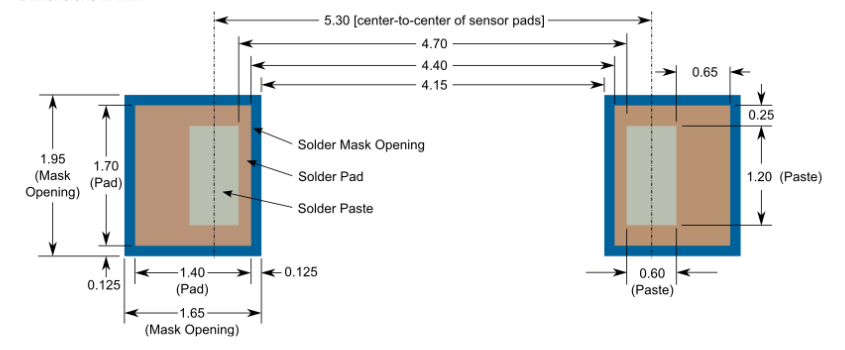
\includegraphics[keepaspectratio, width = \textwidth]{assets/rm3100_foot.png}
		\caption{RM3100 recommended custom footprint configuration}
	\end{figure}
	
	
	
	\textbf{How important are footrpints?}
	A lot of problems originates from poor library implementation. So, it would be wise to always review your libraries. Precisely, check each pad if it is properly assigned for each type of layer (e.g. copper, solder paste, soldermask). Sometimes ready footrpints offered by third party libraries might have some issues like assigning copper areas as a drawing (no electric connection) that can cause many problems. This actually happened in the EPS's board. The drawing had the exact same color with the layer associated with the copper one, so it was very error-prone! For the mistakes made in the engineering models you can check the AcubeSAT-OBC-EC-012.
	
	%If you want to learn more about footprints, there is a nice extensive \href{https://www.youtube.com/watch?v=cMxXea16Hxc}{youtube video} by Robert Fenerec.
	
	\subsection{3D models}
	
	3D models help a lot with the visualization and can be used for debugging. For instance, by viewing your board in 3D, you can inspect if objects are overlapping and if everything fits together. This of course can be done in the PCB layout enabling the layer that is dedicated for the mechanical dimensions (if your footprint contain the required data) like the Courtyard in KiCad, as we have mentioned previously.
	
	\section{Fabrication data}
	
	\subsection{Manufacturing data}
	
	Next step after the finished design is the bare board fabrication. For this purpose, the generation of files with special format called \textbf{Gerber} is the de facto standardized way to connect manufacturers and designers. Each EDA tool has the option to generate these type of files. In short they contain information about the copper of each layer of the PCB, the soldermask and the silkscreen. The \textbf{NC} (Numeric Controlled) \textbf{drill files} are also generated along with the Gerber ones to specify the data for the drilling machines to create the holes of the PCB.
	
	% source, easy googling
	%Any tips and trick for the Gerbers? XY coordinates and origin?
	
	\subsection{Assembly data}
	
	Each assembly house requires certain formats about the data requested for the process, so some differences might exist among them. Assembly data is typically referred to the following:
	
	\begin{itemize}	
		\item Bill of Materials (\textbf{BOM}). The materials used for a cooking recipe! It is usually a csv file that lists everything that the assembler needs to know about the reference designators (component identifiers) and the manufacturing part numbers of the ordered components. Be careful with the default generated format from the EDA. It should be adjusted to the assembly house requirements.
		\item Component \textbf{location} and \textbf{orientation}. For KiCad, this is satisfied by the "CtrYd" (Courtyard) and the "Fab" layers respectively.
		\item Solder \textbf{paste} location. The paste data is used to manufacture an SMD stencil required for reflow soldering. It is a dedicated layer in the EDA tools (for KiCad "Paste" layer). The solder area is almost equal to the size of the pad.
		\item For automatic assembly, specific position files readable by Pick and Place machines are needed, the so called \textbf{X,Y files}. These provide information about the component position and orientation (.pos extension file for KiCad).
		\item Files with location data for the tests points (\textbf{test fixture}), if testing is integrated in the assembly process.
	\end{itemize}
	
	%\href{https://www.seeedstudio.com/blog/2019/06/12/how-to-generate-assembly-files-and-why-they-are-important/}{source}
	
	\begin{figure}[h!]
		\centering
		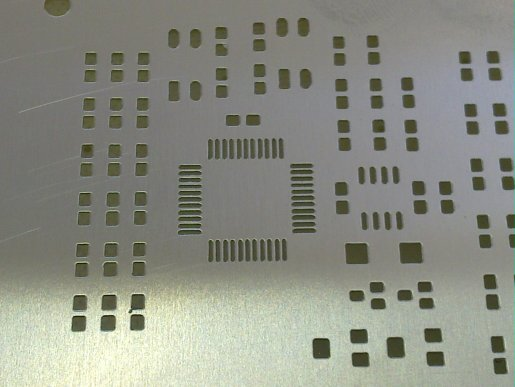
\includegraphics[keepaspectratio, height = 0.25\textheight, width = \textwidth]{assets/solder_paste_stencil.jpg}
		\caption{Stencil by \href{https://www.itmconsulting.com/?product=stencilpro-3-0-stencil-aperture-calculator}{source}}
	\end{figure}
	
	\section{Identifying the design}
	
	%Distinguish the lumped model and the distributed model? When we need to worry about transmission line theory? When circuit theory isn't adequate for designing? What about the digital spectrum, not sine waves? Rule of thumb related with wavelength and propagation speed? Logic levels and rise time? Bandwidth, skew rate. Should I keep in mind these values for filter design and when to apply filters? Frequency response of the components selected must be reviewed? 
	
	Let's start talking about the challenging part of PCB development cycle, the \textbf{design}. All the problems of the PCB can be categorized to \textbf{Signal Integrity} (SI): "involving the distortion of signals", \textbf{Power Integrity} (PI): "involving the noise on the interconnects and any associated components delivering power to the active devices" and Electromagnetic Compatibility\footnote{Usually Electromagnetic Interference (EMI) is referred to the cause of the problem and EMC is referred to the solutions}(\textbf{EMC}): "the contribution to radiated emissions or susceptibility to electromagnetic interference from fields external to the product". These definitions aren't very helpful and sometimes problems of one category may overlap with the another but we are going to investigate them more in the DFP section.
	
	%In general for a long time interconnections of PCB isn't considerable for electrical performance but this changed as the frequency is getting higher. The question is when signal integrity becomes a problem? This is has no clear answer but in general if you are in the MHz region you should start taking high speed guidelines into account.
	
	For now, it should be noted that it is very important to distinguish in the design the existence of transmission lines. They are a subset of the root cause of many problems regarding signal integrity (reflection and the associated side effects) and you will understand why soon.
	
	\textbf{Introduction to distributed model and transmission line theory. }
	Electromagnetism phenomena can be divided to 1) high power and low frequency (electric machines and plants, transformers) and 3) high frequency and low power (mobile devices, modern systems). The focus in this report will be on the second part, so let's take a look on why high frequency really matters? Is actually the frequency the root cause of circuit issues?
	
	In the PCB industry, designers for a long time in the low-frequency era neglected the \textbf{electromagnetism} and build their designs according to its \textbf{abstract} and less complicated version, the \textbf{circuit theory}. The so called traditional \textbf{lumped} model is based on principles such as 1) everything can be modeled via resistors, capacitors, inductors 2) everything happens instantly (there aren't time transients) and 3) interconnections that connect components are equipotential surfaces. This abstract model is a very efficient and practical method to make your application functional without worrying with the complex nature of electromagnetic fields. But as technology is progressing and things are getting smaller and signals are getting faster, the electromagnetic phenomena can not be neglected anymore. This is where \textbf{transmission line theory} along with the wave properties are coming to the surface, that connect the electromagnetism with the circuit theory and introduces the \textbf{distributed} model. According to this model, circuit theory can also be a great tool in high speed applications but with some modifications. Now the tracks that carrying signals can't be treated like equipotential surfaces but as an RLC circuit that extends as a function of the length of the track (image). This result to a much different electric behavior and should be consider. 
	
	%But of course this isn't the only thing that needs to be addressed and progressively more concerns will be mentioned (check design for performance for high speed applications).
	
	%Trying to explain what is reflection, what is radiation. What are the basic concepts of transmission line. Reflection coefficient, standing waves and so on. I am not sure if I am good at this. Maybe wikipedia will help for the generic stuff that I am interested. Interesting thing about antenna impedance is that the goal of the antenna is to have real part and no imaginary part that actually store energy. This happens in fractions of wavelength. The antenna is in resonance. That is why impedance transmission are real. But also 
	
	%\textbf{A very quick introduction about transmission line theory and electromagnetic radiation}.
	This different electric behavior is related with the fact that signals are starting to act like waves. But why and how?
	Waves in nature have some fundamental characteristics. The \textbf{wave} nature of voltage signals is starting to take shape when frequency is very high and length of the interconnections is such that fractions of wavelength can fit to the conductive traces. Just like ocean waves and ropes reflect when they meet an obstacle, a voltage signal can potentially reflect back to the source. A very nice \href{https://www.youtube.com/watch?v=DovunOxlY1k}{video} by AT\&T can help a lot with the visualization to consolidate the analogy! These reflections is the cause of the important aspect of impedance matching. In the PCB case, they can be observed when there are discontinuities (impedance mismatch) regarding the geometry of the conductive path along the way that the signal propagates. Another feature that needs to be considered is the \textbf{radiation} aspect. When charges accelerate, electromagnetic fields are taking shape. The higher the frequency, the shorter the rise time, the faster the acceleration, the greater the radiation. The goal of the transmission lines is to guide the energy with maximum power transfer, zero reflections to an antenna and without radiating energy. So we could summarize that in high frequencies, voltage signals behave like waves and the charge acceleration radiate electromagnetic energy that it can be coupled to undesired pathways if we don't pay attention. We will mention in the section PCB guidelines, more about the problems and the solution regarding high speed signals.
	
	But why transmission lines can be bad? What are the transmission line effects? They can cause timing issues due to the delay of the signal to reach from the driver to the source (tuning traces) and reflection issues such as false triggering, ringing, more EMI and crosstalk, overshoot, distortion etc. As it seems transmission lines can affect severely the signal integrity so we need first to identify them and secondly to address the problems of reflection and delay with impedance matching, proper termination and tuning traces (section DFP).
	
	%There is always radiation. The problem is when it is significant. Energy of radiation is proportional to frequency and inversely proportional to wavelegnth. The shorter the wavelength, greater radiation. The best way to fight the radation is the retunr path for field cancellation.
	
	%In the best case scenario transmission lines should not radiate. To achieve something like this the reference signal, the return path should be close to the signal to cancel the EM fields.
	
	%Don't forget to include why transmission theory isnt bad, antenna and the applications! Reflection cause ringing, radiation can couse coupling and son and these are negative side effects in signal integrity. Why is bad and why is good. As the frequency is getting higher then the EM waves are like dogs that are burking and they can't wait to unleash them to run. The goal is to guide the EM waves and not let them distribute to unintentional pathways. The goal is to guide energy!
	
	Sometimes we are very good at learning individual things but connecting the dots is equally important. A recommended book to connect electromagnetism and circuit theory about electronics is by Ralh Morrison "Fields and electronics". It is very important to start thinking in fields and space rather traces that carrying signals. Viewing traces as the boundary of the space, is more helpful as a designing mindset in the AC world.
	
	%This paragraph is more design oriented, not suitable for the introduction. The impedance matching is referred to such and such. (Be careful when changing the medium!) Check all about circuits for sure. But why reflections are actually bad? Because a portion of the desired energy will be eventually delivered to the load causing circuit failures (logic failures in the digital world). The load didn't receive at a particular time frame the expected voltage. The reflections that are going back and forth may not attenuate until the beginning of the next input signal causing many problems, is this bouncing effect?
	
	\subsection{To be or not to be a transmission line}
	
	A very important question that a designer should ask in the early phase of the decision making about the designing strategies is \textbf{when should I worry about transmission line theory?}\footnote{Transmission line mainly can be referred to any pair of signal and return conductors. In this case we worry about the reflection aspect of transmission lines.} To answer this question we need to know: 1) The propagation velocity of the signals of interest, so the constant of the material that the EM fields are propagated through. In our case we need the dielectric (typical FR-4) one of the PCB. 2) The frequency of the signal that can determine afterwards the wavelength. Wavelength is quite interesting because it is referred to an oscillation, a wave, a sinusoidal function. Circuits are often described by how they respond to sine waves of various frequencies (by Ralph). What happens to the non-sinusoidal inputs though (e.g. square waves)? How to analyze them? 
	
	%Should we also distinguish analog and digital signals? Are analog signals waves, it is a signal and what is its frequency spectrum? We will stick to the wave analysis and the non sinusoidal inputs. For analog the wavelength is the criteria and for analog the rise time!
	
	
	
	%A list with different rule of thumbs about when to worry about reflection and stuff:
	%\begin{itemize}
	%	\item Page 21 by Transmission line analog and digital, divide by ten
	%	\item Altium live RF series, I think something about twenty
	%	\item Managing signal integrity, use time for reference. Dont forget to mention comparable 
	%	\item Ralph Morisson? Actually no rule of thumb, only how to approximate square wave with continuous wave, but I don't see this very often.
	%	\item Eric Bogatin? page 595
	%	\item Wikipedia claims divide by ten
	%	\item Daniel Beerek by 7 in his live thing
	%	\item Gioultsis by 100.
	%	\item Mark montrose divide by 20.
	%	\item circuit companion divide by ten
	%\end{itemize}
	
	%We are going to summarize the above with the following statement:
	%This rule of thumb should not be taken too seriously. Designer may faced transmission line effects even in cases of $\lambda/40$ or can ignore them until the length if comparable with $\lambda/4$. It depends on the acceptable noise margins, the sensitivity of the circuit and the tolerances. So the best response for when designers should worry about these effects is \textbf{When these become important to the design}. In other words the real issue that needs to be considered is how much reflection can the circuit tolerate and still be functional? 
	
	First about the sinusoidal ones, for the transmission line model (microstrip, depicted figure 3), using the equation $ c = \lambda*f$ and knowing the frequency we can calculate the wavelength in free space ($c = 3*10^8$, the speed of light). Including the dielectric constant of the medium the wavelength of interest is $\lambda_d = \lambda/\sqrt{\epsilon_r}$\footnote{This formula is valid in a stripline environment that the field is surrounded by the dielectric. In the microstrip one the effective dielectric should be used due to the air. Propagation velocity of stripline is a stricter rule than the microstrip though.}. For the typical dielectric choice FR4 in PCBs, the constant is $\epsilon_r = 4.5$ (velocity factor, $1/\sqrt{\epsilon_r} = 0.47$).
	% source for the above is circuit companion page 46, also this \href{https://www.youtube.com/watch?v=bVdwu1IoX4k}{guy} does the same thing
	%sometime about propagation velocity they include the permeability. But this is 1, according to \href{https://blogs.mentor.com/hyperblog/blog/tag/velocity-of-propagation/}{this}
	It is worth mentioning that \textbf{it isn't the frequency} that really matters, it is about comparing the length of the tracks that carrying the signal (voltage) with its wavelength. When these two are "comparable", then the designers need to incorporate in their thinking the transmission line theory. To define what is comparable, a rule of thumb well know in the industry with some differences among the references is that the length of the line should not be under $\lambda/10$! For example for a 100MHz signal with FR4 as medium, the length of the tracks should kept under 0,141 m for a transmission-free design! \textbf{But this rule of thumb should not be taken too seriously}. Designer may face transmission line effects even in cases of $\lambda/40$ or can ignore them until the length is comparable with $\lambda/4$. It depends on the acceptable noise margins, the sensitivity of the circuit and the tolerances. So the best response for the question when the designer should worry about transmission line effect is: \textbf{When these effects become important/noticeable to the design}. In other words the real issue that needs to be considered is how much reflection and coupling can the circuit tolerate and still be functional? 
	%But don't take this rule of thumb too seriously, you need to include the circuit tolerance too? page 595 for eric bogatin. An overview of the acceptable noise margins of the logic families and the circuit tolerances will determine how much reflection can handle and the circuit still remains functional. In other words, \textbf{how much reflection can my circuit tolerate and still be functional?} 
	
	%\textbf{Distributed element circuit} is the term that you want to design microwave capacitors and inductors using only copper, stubs and so on without passive components.
	
	%About the distributed model wiki and \href{https://www.allaboutcircuits.com/technical-articles/transmission-lines-from-lumped-element-to-distributed-element-regimes/}{all about circuits} claim that isn't only about the wavelength and the reflection, but it is about the tolerance of the devices. A reflected small percent of the initial may be a very important difference to the operating device. So it depends on the circuit sensitivity.
	
	%For the non sinusoidal, we need to define rise time, skew rate, slope and so on and logic levels. Then the road is better.
	
	\begin{figure}[h!]
		\centering
		\begin{minipage}[b]{0.4\textwidth}
			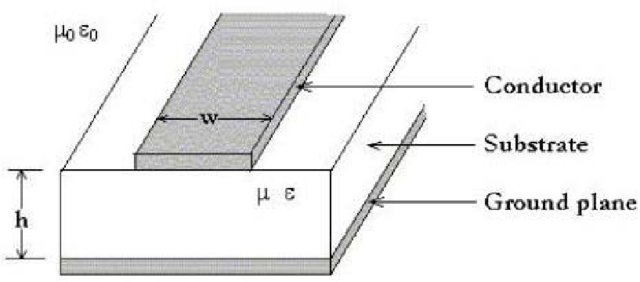
\includegraphics[width=\textwidth]{assets/microstrip.jpg}
			\caption{\href{https://www.researchgate.net/publication/337629930_Design_of_24_GHz_Microwave_Bandpass_Filter}{source}}
		\end{minipage}
		\hfill
		\begin{minipage}[b]{0.4\textwidth}
			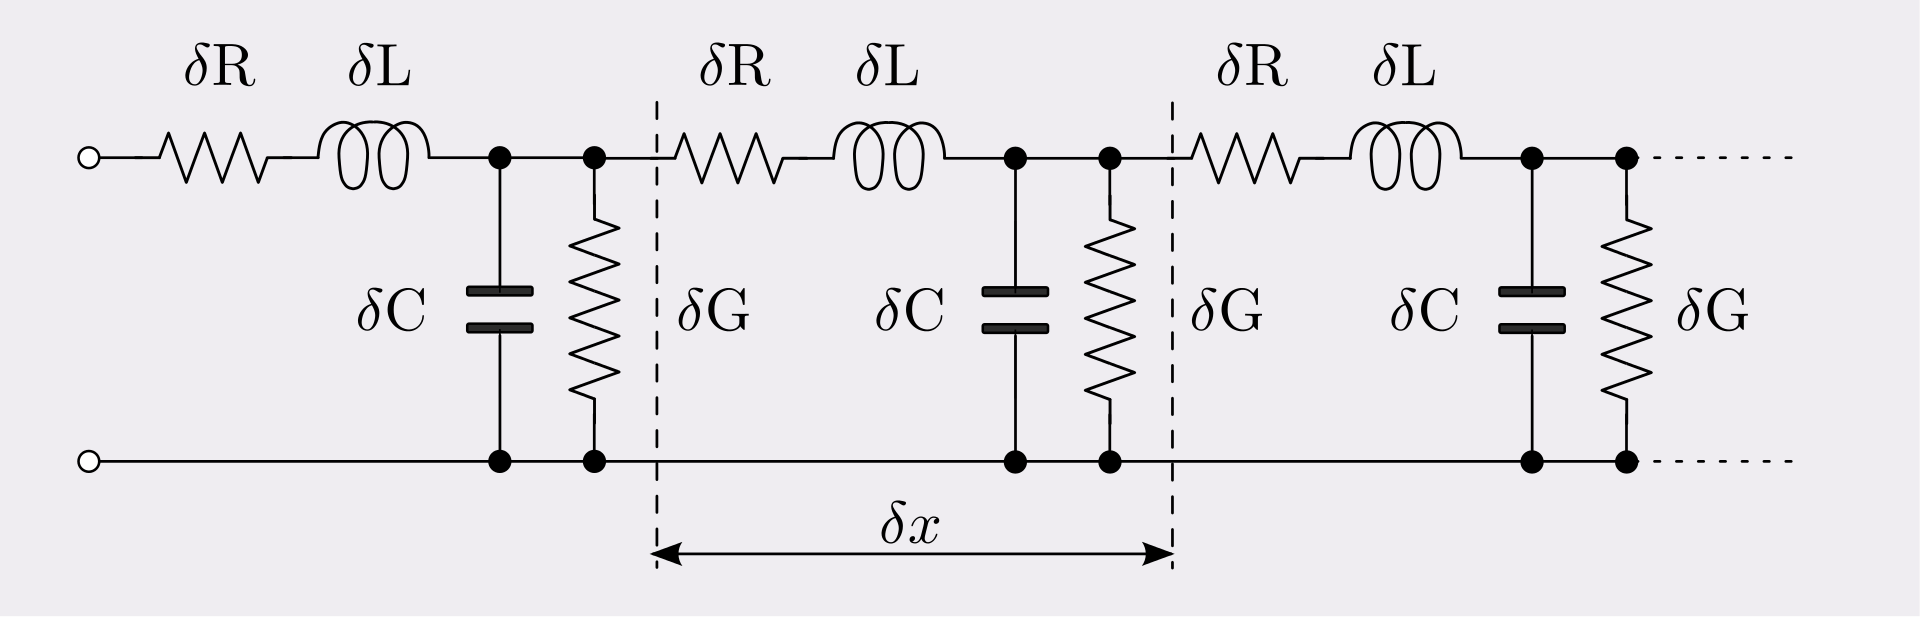
\includegraphics[width=\textwidth]{assets/distributed_model.png}
			\caption{\href{https://en.wikipedia.org/wiki/Primary_line_constants}{source}}
		\end{minipage}
	\end{figure}
	
	
	\subsubsection{Digital signals}
	
	Non sinusoidal signals can be analyzed as the sum of sinusoidal ones (fourier transfrom). This is a very powerful concept that can connect the sine wave analysis with any signal of interest. A very common non-sinusoidal signal with great interest in the digital world is of course the \textbf{square wave} (actually the trapezoidal) and this will be the base to understand the analysis for non-sinusoidal inputs.
	
	\begin{figure}[h!]
		\centering
		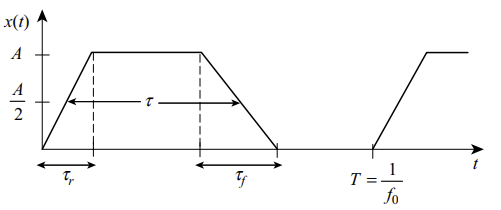
\includegraphics[keepaspectratio, width = \textwidth]{assets/clock_signal.png}
		\caption{Typical digital clock by Transmission analog and digital book}
	\end{figure}
	
	%But treating a signal as very large sum (actually infinite) of sine waves is quite troublesome, maybe we can approximate it with a single sine wave, knee frequency and so on, \href{https://resources.altium.com/p/why-there-transmission-line-critical-length}{source}. About approximating the pulse response Ralph Morisson has something to say in the section about spiked and pulses. Also you could check the Daniel Beerek in the Altium Live, he said something similar.
	
	The \textbf{response} of a pulse can be analyzed as the sum of the responses of the sine waves that constitute the pulse. With that in mind, a pulse response contain a large amount of information regarding a range of frequencies. So when dealing with such inputs, the analysis of the circuits is getting more complex because the designer needs to think not one sine input but a frequency spectrum. In the case that we want to determine when the length of the trace is critical for mitigation of electromagnetic phenomena, we will introduce the terms \textbf{rise time} (time domain) and \textbf{bandwidth} (frequency domain) (and \textbf{skew rate}).
	
	What is rise time? Rise time usually referred as the time needed to go from 10\% of the amplitude of the signal to the 90\%. But why? I think I have some stuff written in the report check also the douglas brooks book.
	
	In high speed design, it can be approximated by the 10\% of the clock period ((eric bogatin page 113)). In some cases like FPGA and ASIC, rise time can reach 1\%! However, wafers could be designed in such a way that can affect it dramatically despite operating in low frequency. It's a function of the logic family and the chip technology.
	%(Rise time is what actually matters because this is where high frequency components exists and this will determine the threshold for the designing strategy of incorporating high speed guidelines to our design.) 
	Another rule of thumb claims that it can be estimated as the\textbf{ 7\% of the period}. As we said, most of the times rise time will be 10\%, but is better to underestimate than overestimate. Rise time is essential as an input for design strategies and the why will become clear soon.
	
	
	From the time domain we will jump to the frequency one. As we have said, a pulse can be described as an infinite sum of sinusoidal functions, but the \textbf{infinite} term is quite troublesome for the analysis. Do we need all the harmonics for an adequate representation of a pulse? We can actually neglect some frequency components due to the very low magnitude. In other words when they are not significant. Hence we can define \textbf{bandwidth}\footnote{The term bandwidth is used as the highest frequency component because in the frequency spectrum digital signals start at the DC} as the highest sine-wave frequency component that is significant in the spectrum. But how to define the "significant". There are some variations regarding this:
	
	\textbf{First} approach by Clayton R. Paul. If we are going to plot the frequency spectrum of a trapezoidal signal we can observe that while the frequency increases, the magnitude decreases. Precisely in the figure 8 we see that after the breakpoint $1/\piτ$ the levels of harmonics are rolling off at a rate of 20dB/decade, then at the second breakpoint at a rate of 40 dB/decade. If we go past the second one by a factor of about 3 to the frequency that is the inverse of the rise and fall time, $f = 1/τ_r$ then the levels of the component we will be reduced further by 20dB. This breakpoint will be $f = 3 * 1/\piτ_r \approx 1/τ_r$.  Hence we can claim that above this frequency the components will be negligible and we define the bandwidth of the trapezoidal clock as:
	
	\[\text{BW} = \frac{1}{τ_r}\]
	
	\begin{figure}[h!]
		\centering
		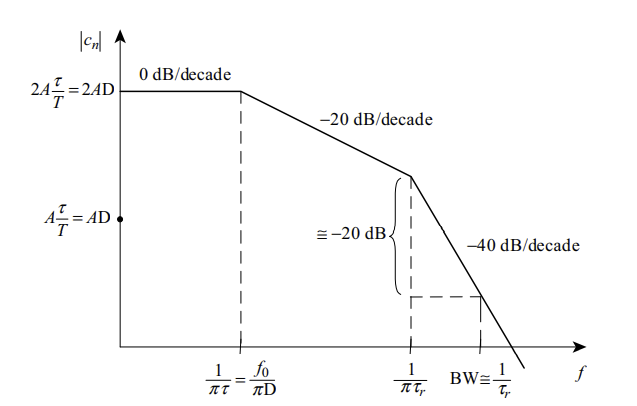
\includegraphics[keepaspectratio, width = \textwidth]{assets/magnitude_clock.png}
		\caption{Bounds on the spectral coefficients of the trapezoidal pulse train for equal rise and fall times}
	\end{figure}
	
	\begin{figure}[h!]
		\centering
		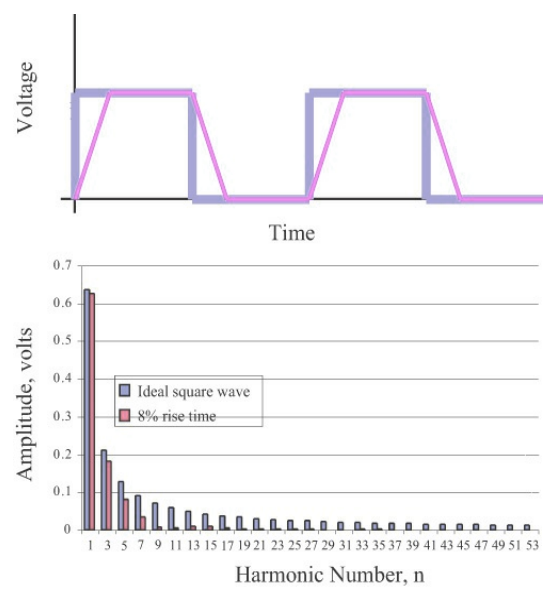
\includegraphics[keepaspectratio, height = .4\textheight, width = \textwidth]{assets/square_n_trapezoidal.png}
		\caption{By eric bogatin}
	\end{figure}
	
	\textbf{Second} approach by Eric Bogatin. Let's try to re-create an ideal square wave (zero rise time) by adding harmonics. We can see in figure 10 that whenever we add more harmonics, the rise time becomes shorter and a trapezoidal signal is starting to take shape. Eventually the trapezoidal could become an ideal square if infinite harmonics were added. We are not interested in an ideal square, but in the trapezoidal ones that resembles the digital signals. So, for these signals, from which frequency and after, adding harmonics isn't significant anymore? Let's take the harmonics of an ideal trapezoidal signal and a square one. We are looking for the harmonic of the trapezoidal that its power is 50\% less than the power of the same harmonic of the square wave or when the amplitude is 70\% less. Then this harmonic is the highest frequency component and thus the bandwidth is defined.
	
	\begin{figure}[h!]
		\centering
		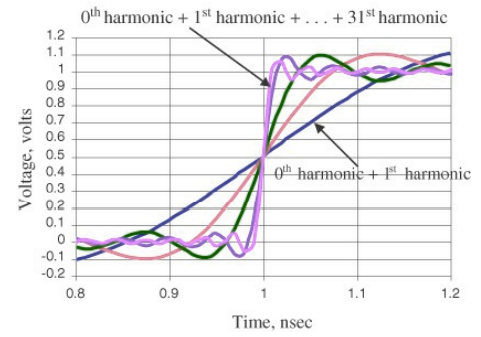
\includegraphics[keepaspectratio, width = \textwidth, height = .3\textheight]{assets/harmonics.png}
	\end{figure}
	
	So we are actually using the harmonics of a square wave to build a trapezoid signal but the the highest frequency component is found by comparing the amplitude or the power of the harmonics of a trapezoidal and an equivalent square wave. According to this there is a linear relationship between bandwidth and rise time depicted in figure 11. Mathematically can be described as:
	
	\[\text{BW} = \frac{0.35}{\text{Rise time (10\%-90\%)}}\]
	
	\begin{figure}[h!]
		\centering
		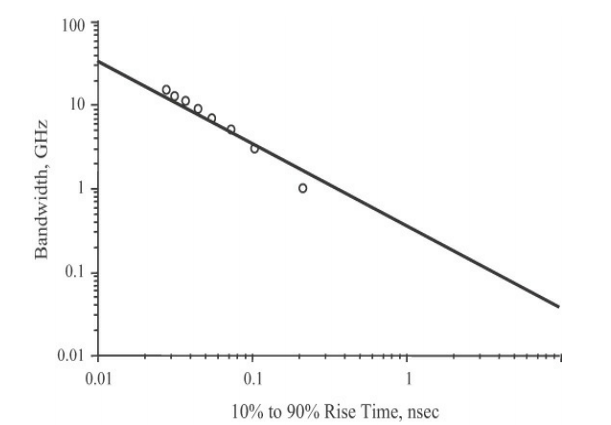
\includegraphics[keepaspectratio, width = \textwidth, height = .3\textheight]{assets/band_rise.png}
		\caption{Linear relationship between bandwidth and rise time of trapezoidal signal}
	\end{figure}
	
	
	\textbf{Third} approach by Howard Johnson. Let's take the power spectral density of the signal depicted in figure 11. We can see that from the clock frequency until the so called knee frequency we have a 20dB/decade slop. Beyond knee frequency the amplitude rolls of faster. At this particular breakpoint the spectral amplitude is down by half (-6.8 dB) below the 20dB/decade slop. Thus we can claim that most of the energy in digital pulses is concentrated to the frequencies from the DC to the knee frequency. How to find the knee frequency based on the rise time, though? There is this formula:
	
	\[F_\text{knee} = \frac{0.5}{\text{Rise time (10\%-90\%)}}\] 
	
	
	\begin{figure}[h!]
		\centering
		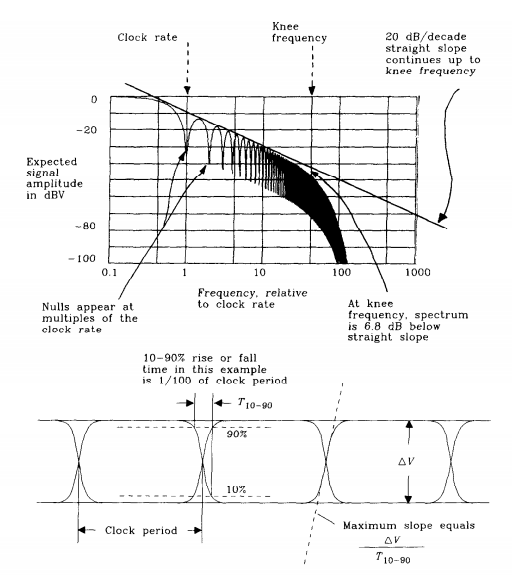
\includegraphics[keepaspectratio, width = \textwidth]{assets/eye_spectra.png}
		\caption{Eye diagram of a digital signal and its power spectral density}
	\end{figure}
	
	With these three methods we are able to measure the highest significant frequency component of a digital signal. All the sine waves from DC to that frequency is important for our design, so the transmission line should be able to handle this range of spectrum. If a portion of this frequency range falls of to the category of transmission line as it was defined with the rule of thumb for the wavelength per sine wave, then high speed design guidelines should be definitely considered. 
	
	\subsection{A transmission line problem}
	
	Let's see an example to comprehend the transmission line problem in digital signals. We will be based to the first approach to estimate the bandwidth. So, let's assume that the voltage source depicted in figure 12 is a clock waveform of 5V, 50 MHz, 50\% duty cycle, rise time 0.5ns and the length of the interconnection is 2 in (0.0508m). The bandwidth of this waveform is
	
	\[\text{BW} = \frac{1}{0.5 * 10^{-9}} = 2 \text{GHz}\]
	
	Let's calculate what should be the frequency of a sine wave in order for the interconnection to act like an electrical short according to the rule of thumb of $\lambda/10$. So we set $\lambda/10 = 0.0508 \text{m}$. We assume FR4 as dielectric (($1/\sqrt{\epsilon_r} = 0.47$)), so
	
	\[\lambda/10 = \frac{c}{f * \sqrt{\epsilon_r} * 10} = \frac{3 * 10^8}{f * 10} * 0.47 \rightarrow f = \frac{3 * 10^8}{0.0508 * 10} * 0.47 = 277 MHz \]
	
	We have a signal that its frequency clock is 50MHz and the bandwidth 2 GHz! For the range 277MHz - 2GHz the interconnection isn't electrical short and the distributed model should be introduced. So definitely for this, transmission line effects should be taken into account. As you can see the clock frequency of 50 MHz doesn't tell much for the criteria to be or not be transmission line... 
	
	\begin{figure}[h!]
		\centering
		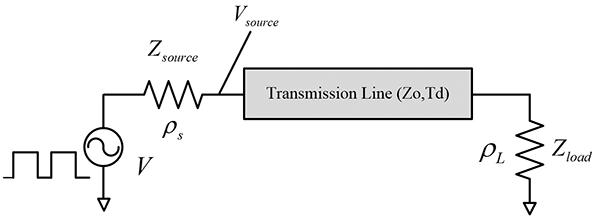
\includegraphics[keepaspectratio, width = \textwidth]{assets/transmission_input.png}
		\caption{\href{https://incompliancemag.com/article/an-overview-of-transmission-lines-in-electronic-systems/}{source}}
	\end{figure}
	
	In a different way we could calculate at which length of the interconnection you should start worrying and similarly we have (f = highest frequent component, BW = 2 GHZ):
	\[\lambda/10 = \frac{c}{f * \sqrt{\epsilon_r} * 10} = \frac{3 * 10^8}{2*10^9 * 10} * 0.47 = 0.007 \text{ m} = 7 \text{ mm} \]
	
	Thus for length below 7 mm, we can estimate that the interconnection won't behave as a transmission line.
	
	\subsection{Lumped vs Distributed}
	\textbf{Another method} proposed by Howard Johnson for identifying \textbf{lumped vs distributed systems} is the following:
	
	Everything takes times and nothing can travel faster than the speed of light. So the signal from the driver to reach the load will take some time, there will be a delay. This delay is proportional to the length of the trace, but during the delay there is a possibility depending the rise time to fit a portion of the signal to this segment of trace and wave nature is coming to the surface. The rising edge is the factor that determines if the signal can fit to the segment of the trace. We can defie the length of the rising edge (in m) as:
	
	\[l = \frac{T_r}{D}\]
	
	where $T_r$ is the rise time (10\%-90\%) in ps and D is the delay, how much time took for the signal to move per unit length (ps/m).\textbf{ For circuits smaller than $l/6$ are lumped}.
	
	\begin{figure}[h!]
		\centering
		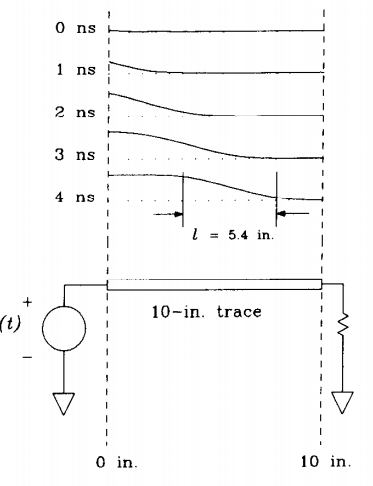
\includegraphics[height = .3\textheight, keepaspectratio, width = \textwidth]{assets/rising_edge_length.png}
		\caption{Length of the interconnection and the length of the rising edge}
	\end{figure}
	
	%It should be noted that high frequency harmonics attenuate significant more than the lower ones due to conductive and dielectric loss especially when traces are long. Less high frequency components, the rise time is increasing and the bandwidth is decreasing, resulting in a much different wave that the initial one. 
	
	%\subsection{Summary}
	
	%The sharper the edge, the shorter the rise time, the bigger the bandwidth, transmission line effects are emerging. Transmission line phenomena are related with reflection and radiation (coupling, crosstalk). How these can actually affect the design and what we can do about them? We will see in the next section.
	
	%more radiation and emissions. The following equation is an approximation and it is based on\textbf{ 50 percent duty cycle}, rise time and frequency of a square pulse. The rise time is the fundamental contributor of the digital spectra and not the frequency of the digital signal itself. 
	
	%But why having transmission line is bad? Actually it isn't bad at all, there are many applications based on the reflection and the radiation. But the point is to identify these characteristics and mitigate them when it is needed or make use of them. In our case, we don't design antennas so we need to suppress radiation and guide the field where it is supposed to go, to the desired load.
	
	%Our goal is to not have high frequency components to avoid reflections and radiation or to lower their magnitude to become insignificant. For example if we don't take into account impedance matching to mitigate reflection, the ringing will cause to make negligible high frequency components to significant.
	
	%Nice to know: The energy associated with a wave is directly proportional to its frequency. Hence, the higher the frequency, the shorter the wavelength and the higher the energy of the wave. It is all about the energy of radiation, amplitude and frequency.
	
	
	%\section{PCB design guidelines or challenges, issues, problems and solutions}
	
	
	\section{Design for Performance}
	
	%As the frequency gets higher the impedance is dominated by reactance and not resistance. Smaller loops can significantly reduce the inductance, so the return current path following the rule of the least impedance, will travel below the signal trace. That is why slots and switching layers is the root cause of many problems. If trace of the length is one time important then making the loop area is ten times important (\href{https://learnemc.com/pcb-layout}{source})
	
	%In the case of transmission lines should be also consider the impedance matching and tuning the traces for time critical signals. I am not sure if high speed is and distributed model is equivalent to transmission line. In other words if I keep my interconnects very short to meet the above criteria, do I need not to worry about nothing, not even planes and so on. Common mode noise is radically different than these but what else?
	
	%In this section (Design for Performance\footnote{I am not really sure if this is an accurate term regarding the PCB literature. The purpose is somehow with this term to group most of the PCB electrical issues.}) we will try to give an overview of techniques regarding the electrical performance of a PCB design for the purpose to meet the requirements and the specifications, especially when we are dealing with high speed constraints. 
	
	\textbf{Design for Performance} is referred to electrical performance and it becomes crucial in high speed applications when a lot of guidelines should be implemented to meet the requirements. 
	High speed design is something that you can't explicitly define. We mentioned some rules of thumb for the transmission line and the distributed model, but in general in the MHz region and above you should treating lines with a careful mindset\footnote{ It is should be noted that the voltage of the signal is quite important for the radiation. A fast rising time of a 5V signal would have more energy than a 3.3V. This is why the \textbf{slew rate} (how fast the voltage change) can be actually a better indicator of signal criticality.}. It should be noted that every pair of signal and return path can be defined as a transmission line. We may keep the interconnections small and not having reflections and this is good but just a subset of the signal integrity.
	
	\textbf{Question}: Even if I have very short rise times that means trouble, but the pin changes its state not very often (it isn't periodic like the clock that change its time very frequently), can I assume that it isn't a critical signal eventually? \href{https://www.ti.com/lit/an/szza009/szza009.pdf}{source, page 2, PCB design guidelines for reduced EMI}
	
	% Most of the problems in PCB design fall of to these categories:
	First we categorized the problems in SI, PI and EMC. A more practical way to categorize the issues in the design is the following:
	
	%By Eric Bogatin:
	
	%\begin{itemize}
	%	\item Reflections
	%Ringing, enhance the crosstalk, magnitude of higher components become significant
	%	\item Crosstalk
	%	\item Ground and power bounce as a special case of crosstalk
	%	\item Losses. This is referred mostly to the GHz region and we are not so much interested to so high frequencies for this report.
	%	\item Rail collapse in the power and the distribution network
	%	\item EMI
	%\end{itemize}
	
	By Douglas Brooks
	
	\begin{itemize}
		\item \textbf{E}lectro\textbf{M}agnetic \textbf{I}nterference (radiations beyond the board or susceptibility to radiations from outside the board)
		\item \textbf{Reflections} on a single net
		\item \textbf{Crosstalk} between two or more nets, in many ways a special case of EMI
		\item \textbf{Power system stability} 
	\end{itemize}
	
	\subsection{Forget the Ground think Return}
	
	%Eventually the current should return to ground and will try to find a bypass capacitor to do that (\href{https://resources.altium.com/p/should-you-use-your-power-plane-as-a-return-path}{source})
	
	%In high frequency what determines the impedance is not the resistance but the reactance.
	
	In high frequency signals where voltages and currents changing/oscillating, there aren't any shorts or opens like we are used to. Even two conductors with voltage difference separated by a dielectric can act as a very low impedance path and definitely not something that current can't flow (displacement current). Another thing that we need to understand is that \textbf{current flows in loops} and always trying to find the path with the \textbf{lowest impedance} (yes impedance and not resistance. In higher frequency reactance dominates resistance, \href{https://learnemc.com/pcb-layout}{source}). This path will be the adjacent copper area because the loop is smaller, the capacitance is higher thus the impedance is lower. So it is considered best practice to place the ground plane (about planes check this) very close to the signal.
	
	\begin{figure}[h!]
		\centering
		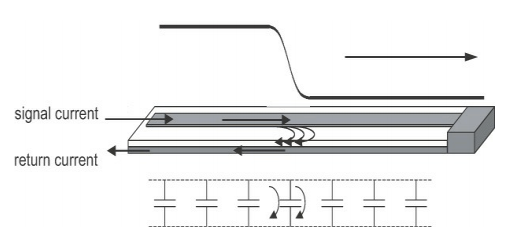
\includegraphics[keepaspectratio, width=\textwidth, height=.2\textheight]{assets/signal_return.png}
		\caption{By eric bogatin}
	\end{figure}
	
	But if we think that everything is fine by connecting the return path to the ground plane, this is where a lot of problems arise. As we have said the current will find the path of the lowest impedance. If for some reason there is copper area between the signal and the ground then the return path will not be in the ground but in the copper between them. In other words the current will follow a radically different route from what we estimated with side-effects such as overlapping currents, crosstalk, distortion! In the end the current should return to ground. So a very important rule is to have an \textbf{an unbroken dielectric} between the signal and the return. 
	
	\begin{figure}[h!]
		\centering
		\begin{minipage}[b]{0.4\textwidth}
			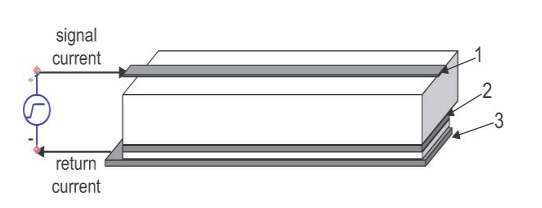
\includegraphics[keepaspectratio, width=\textwidth]{assets/broken_dielectric.png}
			\caption{By eric bogatin}
		\end{minipage}
		\hfill
		\begin{minipage}[b]{0.4\textwidth}
			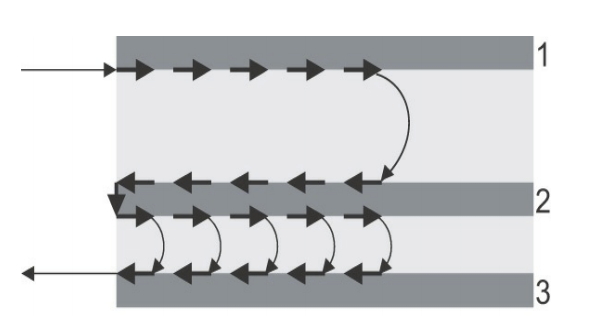
\includegraphics[width=\textwidth]{assets/side_current.png}
			\caption{by eric bogatin}
		\end{minipage}
	\end{figure}
	
	\subsubsection{Changing trace layers}
	
	And if I have to change layers how to follow the rule of the unbroken dielectric? What will be the return path? This is quite interesting actually and in order to visualize it let's inspect the figure 14.	In this figure we assume that layer 2 and 3 are reference planes with the same potential, thus we can connect them using a via. But before talking about the via, we can observe that in the layer 1 and layer 3 the return current follow the principle of the adjacent layer as we expected. The big challenge is what is happening between the 2 and 3, how the current can return? Thus we put the via to provide a path for the return current to transition from the 3 layer to the 2.
	
	Let's now see the figure 15, without using a via and having as planes the ground and the power for the 2 and 3 correspondingly. How the current will return? It will spread out around the clearance created from the hole and will try to make use of the capacitive coupling between the two planes. Why it spreads? For lower inductance and for higher capacitance. This discontinuity though it will increase significant the impedance causing a voltage drop in the ground plane the so called ground bounce. For this case we could place a bypass capacitor near the via that will act as a low impedance path for the current (be careful with the loop inductance, the bypass capacitor eventually may not act as one). We could also minimize the clearance of the hole, making the via smaller to reduce the voltage drop. The distance between the two plates in order to increase the capacitance and lower the impedance should be kept as small as possible.
	
	\begin{figure}[h!]
		\centering
		\begin{minipage}[b]{0.4\textwidth}
			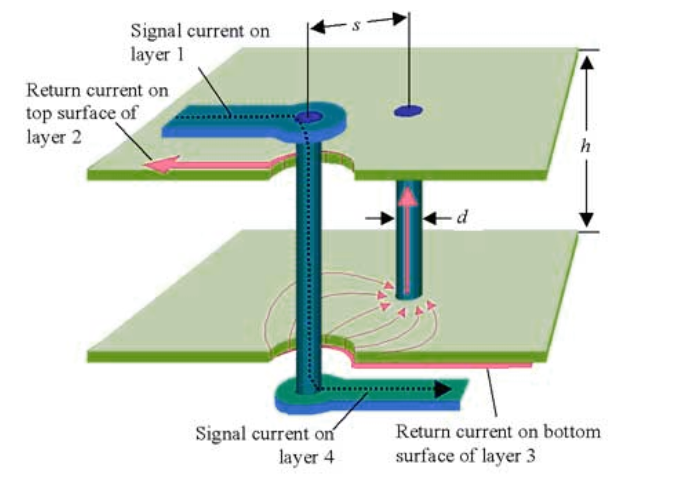
\includegraphics[keepaspectratio, width=\textwidth]{assets/change_layer.png}
			\caption{\href{http://www.sigcon.com/Pubs/news/6_04.htm}{source}}
		\end{minipage}
		\hfill
		\begin{minipage}[b]{0.4\textwidth}
			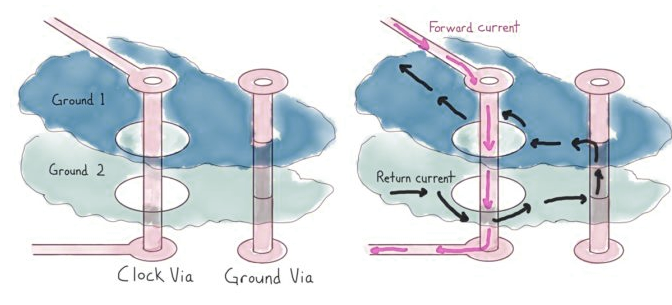
\includegraphics[width=\textwidth, keepaspectratio]{assets/ground_trans.png}
			\caption{\href{https://www.tempoautomation.com/blog/design-to-avoid-emi-problems-keep-clocks-away-from-unintended-antennas/}{source}}
		\end{minipage}
	\end{figure}
	
	\begin{figure}[h!]
		\centering
		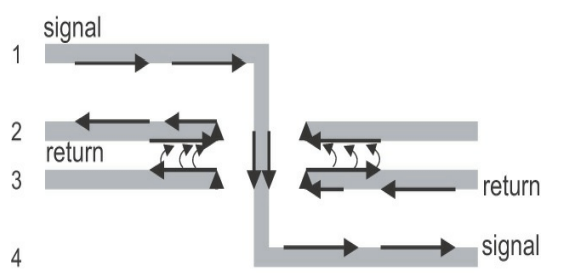
\includegraphics[width=\textwidth, height=.25\textheight]{assets/change_layer2.png}
		\caption{by eric bogatin}
	\end{figure}
	
	
	%The current can't penetrate between the two planes (capacitance between plates isn't enough) and will try to find a way to come back to the ground, probably by a bypass capacitor locates somewhere in the board. A better approach is to provide a return current path close to the one the via that drive the signal to another layer either with an additional via (ground transition vias) if the planes have the same voltage or with a bypass capacitor.
	
	\subsubsection{Slots}
	
	Another thing encountered in PCB designs is a disrupted return path with slots in the ground plane. The return path is disrupted, the current will flow around the loop, thus the inductance increase resulting to more emissions and voltage drop (ground bounce). The field of the signal path during the slot isn't canceled by the return path. To calculate the inductance of these slots for accuracy you could use 3D field solvers. In general the bigger the area of the loop, the higher the inductance and the more the problems. It would be best to avoid slots or don't route signal over them or if you can't do anything you could place a bypass capacitor as a path of low impedance (\href{https://electronics.stackexchange.com/questions/81761/whats-radiating-on-my-pcb}{source})
	
	
	
	\begin{figure}[h!]
		\centering
		\begin{subfigure}{.5\textwidth}
			\centering
			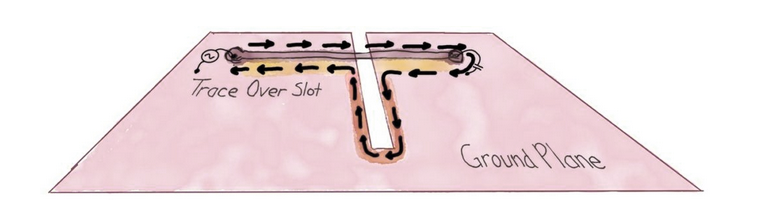
\includegraphics[keepaspectratio, width=\textwidth]{assets/slot.png}
			\caption{\href{https://www.tempoautomation.com/blog/design-to-avoid-emi-problems-keep-clocks-away-from-unintended-antennas/}{source}}
		\end{subfigure}%
		\begin{subfigure}{.5\textwidth}
			\centering	
			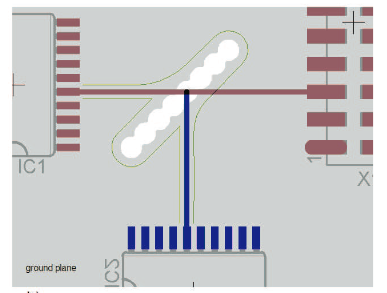
\includegraphics[width=\textwidth]{assets/slot_via.png}
			\caption{Vias clearance cause slots in the ground plane. High speed layout guidelines TI}
		\end{subfigure}
	\end{figure}
	
	Also these type of slots can be created by holes too like vias. If vias are placed very close to each other the clearance will create a gap without any copper between them. This will result to higher impedance that is of course undesired. So be careful with the clearance of the holes. Make them smaller or further the distance.
	
	Now that we analyzed the slots we will introduce another very important rule like the unbroken dielectric, \textbf{the unbroken return path}.
	
	
	\subsubsection{Summary}
	
	What should I keep? Two important rules for high speed design: 1) Unbroken dielectric and 2) unbroken return path.
	%As we have seen , \textbf{identifying the return path} is game changer for mitigating a lot of issues. 
	To put it in another way, you should remember: \textbf{IT IS ALL ABOUT THE FIELDS}. Start thinking in pairs of conductor and dielectric, not per signal trace.
	
	Identifying the return current can solve a lot problems. Where is the source, the load and the return.
	
	%The aforementioned guidelines are a portion of the solutions to mitigate signal integrity regarding the EMI and the rail collapsing noise. More will be mentioned all the way.
	
	The aforementioned guidelines fall of to the category of solutions to mitigate EMI and rail collapsing noise (subset of power integrity).
	
	\subsection{Reflection}
	
	As we have said in the section about the design identification, the signals can have wave nature. Precisely, we analyzed when these kinds of reflections should be significant by comparing the wavelength of the signal with the length of the interconnection. In the case we have transmission lines and reflections, what should we do to avoid problems such as ringing, false triggering, crosstalk and distortion? The answer is \textbf{impedance matching}.
	
	Reflections happens each time the signal face an impedance discontinuity along its way of propagation. These discontinuities can be via, junctions, traces with different geometric shape, connectors, pins of ICs etc. Our goal it to shape a path for the signal with a constant impedance along the way. But we need first to define what is \textbf{characteristic impedance} for a transmission line. It is the constant, instantaneous impedance that the signal looks. It can be defined as the input impedance of an infinite transmission line. It should be noted that there are many formulas that can calculate the characteristic impedance of any type of transmission line. In our case we are mostly interested in microstrips.
	
	
	\begin{figure}[h!]
		\centering
		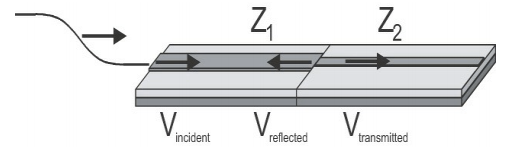
\includegraphics[width = \textwidth, keepaspectratio, height=.3\textheight]{assets/impedance_matching.png}
		\caption{Eric Bogatin}
	\end{figure}
	
	Our goal it to match the impedance of the transmission line with the source impedance of the driver and the load (but actually only for the impedance of the interconnection we have control). Let's suppose that we have a driver, a load and an interconnection (a uniform transmission line without stubs) and we want to design the transmission line so there aren't reflections. First we need to know the source impedance and the load impedance. For a typical CMOS device that drives the signal we suppose that we have impedance of 5-20 Ohms. Similarly for the load we suppose that we have a capacitor. In most CMOS reveivers the capacitance value is very low so it can be approximated as an open circuit. The source impedance can be extracted by IBIS models or by datasheets too. So how we do the impedance match? 
	
	Usually the microstrip traces are routed in such a way adjusting the width to have characteristic impedance \textbf{50 Ohms}. In RF application, with coaxial cables and such, the traces on the PCB are designed with a 50 Ohm characteristic impedance. This is a well know standardized value for cables and RF chips. It is a convention in order to help different vendors to design their products having this value in their minds for impedance matching between different products. But in the case of PCB tracks, the density is very high and designing 50 ohms trace isn't often very convenient. If the design isn't dependent of a coaxial cable or something that forces the trace to be 50 Ohms, can I still use a different characteristic impedance?
	
	The goal it to match the impedance. So if we had a 100 ohm characteristic impedance and the source impedance is 10 ohms, by connecting a 90 ohms resistor in series with the driver then we have impedance matching. However with this configuration, we created a voltage divider and the voltage waveform in the transmission line will be actually half of the intended. But due to the 100\% percent reflection\footnote{When a transmission line is opened from the load end then all the forward signal is reflected back to the source} at the end of the transmission line, the total waveform by adding the reflected will be V volts and when the reflected wave reach the source it will not be reflected back because of the 90 + 10 = 100 impedance.
	
	It should be noted that terminations and impedance matching is a quite huge topic (we didn't even scratch the surface!). It is recommended to read also the documents provided by the vendors that will suggest the best way for the termination of the critical signals. For example, regarding the high-speed USB, the impedance for the differential pair should be 90 ohms.
	
	%\textbf{For purposes of this explanation, CMOS receivers look like very small capacitors that can be considered to be open circuits}, \href{https://www.altium.com/solution/transmission-lines-and-terminations-in-high-speed-design}{source}
	
	% PCB tracks not 50 ohms, \href{https://electronics.stackexchange.com/questions/325143/are-i-o-buffers-of-ics-design-to-have-50ohm-impedance}{source}
	
	%What do we mean that the signal will be absorbed?
	
	%\begin{figure}
	%	\centering
	%	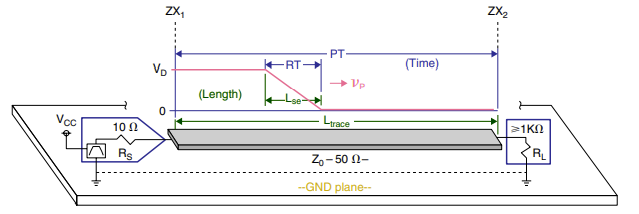
\includegraphics[width=\textwidth, keepaspectratio, height=.3\textheight]{assets/terminating.png}
	%\end{figure}
	
	%If the impedance of the source is a resistor? It is typical for CMOS? The transmission line acts like a voltage divider, so the lower the resistance the more voltage will be applied to the ends of the transmission line. Yes usually CMOS drivers have source impedance and the signal is modeled with a voltage source. Of course we have some kind of voltage drop due to the resistor, not everything go to the transmission line.
	
	If you want to connect multiple receivers then daisy chain routing techniques is recommended in order to keep the characteristic impedance controlled without making branches and stubs.
	
	\textbf{Question}: If I have a via along the interconnection path? What should I do?
	
	\subsection{Crosstalk}
	
	%What are the requirements? How much noise does the board can handle? Interconnection density ? Everything comes with a cost! What are the acceptable noise margins?
	
	%Fringe fields, field that spread, is this far field vs near field
	
	%Coupling happens only when things change.
	
	%You could mention the 20H rule too.
	
	%If we are close to the fringe field region, when voltage, current change then this will cause current to flow through the changing electrics as displacement current and as induced currents from the magnetic fields. 
	
	%Our goals is to minimize the overlap of the fields between two signals: 1) minimize the space between the return path to reduce the spread and further the distance between the signals.
	
	%EM field intensity is inverse proportional with the square root of distance, so the further apart the better.
	
	%It is very important to translate the geometry of the traces into capacitive and inductive noise. Simulation!
	
	%Of course crosstalk get worse if we have reflections without taking into account anything about impedance matching. Actually in general a lot of things get way worse.
	
	When there is current there is magnetic field, when there are charges there is electric field. When current change, magnetic field change and this can induce current to nearby conductors if the magnetic rings spread by the source are shared with them. Because of this mutual inductance and the \textbf{inductive coupling}, noise is produced. This is called switching noise (because happens during the switching part of the current, during the rise time). Opposite current can be induced to the same conductor that created the current in the first place too. The amount of the voltage noised is determined by the total inductance (the total amount of the rings that surrounds the conductor) and of course the rate of change. This is the so called inertia, it takes time to build up current. 
	
	On the other hand when charges are oscillating, they create changing electric fields that can kick charges of the adjacent conductors and current shows up (displacement). This is called \textbf{capacitive coupling} and it is based on the mutual capacitance between two conductors. All of the aforementioned regarding the induced voltages and current when EM fields change, can be described by the notorious 4 Maxwell equations.
	
	The change of these EM fields is actually the root cause of everything. Thus coupling happens during the edges, the rise time. When the coupling is undesired we call it crosstalk. Our goal is to have high capacitive coupling and low total inductance for the signal and the return and low capacitive coupling and low total inductance to unrelated signals.
	
	\begin{figure}[h!]
		\centering
		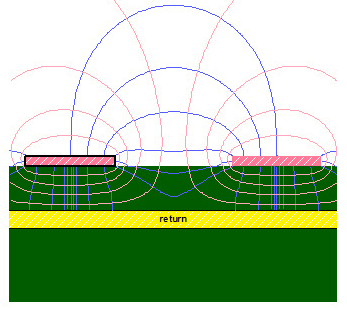
\includegraphics[keepaspectratio, height=.3\textheight, width = \textwidth]{assets/fringe_fields.png}
		\caption{Microstrips, fields overlap \href{https://www.signalintegrityjournal.com/blogs/4-eric-bogatin-signal-integrity-journal-technical-editor/post/402-pop-quiz-use-tight-or-loosely-coupled-differential-pairs-to-reduce-cross-talk}{source}}
	\end{figure}
	
	%As we mentioned in the previous subsections, the current is following the path of the least impedance and this path is located to the adjacent copper area of the signal. But actually let's take a closer look on what is really happening for the purpose to understand how to make use of this induction and to prevent it when it is undesired.
	
	%Forward, backward corsstalk and near and far field.
	In this kind of topic usually authors write about forward, backward and far and near crosstalk. We won't go into too much detail. The concept is that in an environment that we have two microstrips and a signal is propagating to one of them, then there are two directions that induced current can flow, the forward (the same with the signal that caused the coupling) and the backward (the opposite of the signal) and two types of noise, the near (lower in magnitude but last longer) and the far (higher in magnitude but lost shorter). The near is at the start of the trace close to where the signal started to propagate  and the far is at the other end where the signal reaches the destination.
	
	%It should be noted that capacitive coupling is what makes the current to flow to adjacent layer. The inductive coupling is inductive noise, thus we always try to minimize the inductance. I am not sure if this is valid. But in the inductance we mention that in general is noise.
	
	% when the return path is a wide plane, then the capcitive and inductive coupling have the same magnitude. When traces are used for the return, the inductive coupling is far more severre, because the inductance rises radically
	
	In the bottom line there are 4 main things that determine the coupling:
	
	\begin{itemize}
		\item Width.
		
		%The wider the return path, the better, this is why planes are used for ground. Also the bigger the width of the signal, less the inductance and higher the capacitive coupling in the return path but also to the adjacent unrelated signals which is undesired. Space between them is a more important factor.
		
		About the inductive part, the less the density of the current the less the inductance. So increasing the cross section of a conductor also leads to a lower self inductance. This is why ground plane has low inductance too. By increasing the width of a signal, the capacitive coupling between the signal and the plane is increased too.
		\item Space.
		
		Bring the return plane as close as possible to the signal to minimize the area of the loop (field cancellation, lower total inductance, less crosstalk and emissions) and further the distance of unrelated signals as much as possible, considering the density of the interconnection and mechanical constraints. We know that field intensity is proportional to the inverse square of the distance.
		
		But why by minimizing the space between signal and return is better? As we can see there is field cancellation and the total inductance is low. 
		
		\begin{figure}[h!]
			\centering
			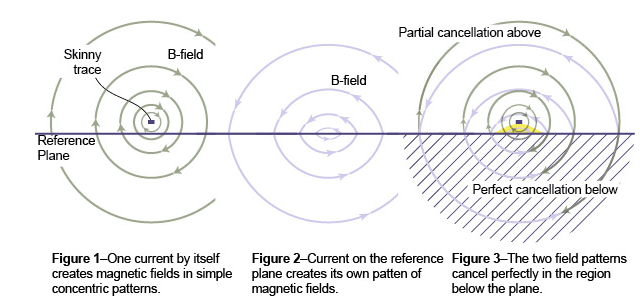
\includegraphics[keepaspectratio, width = \textwidth]{assets/field_cancellation.png}	
			\caption{Field cancellation}, \href{http://www.signalintegrity.com/Pubs/edn/FieldCancellation.htm}{source}
		\end{figure}
		
		\item \textbf{3H rule}.
		
		There is also the 3H (three times the H) rule that indicates the required distance between an aggressor and a victim trace. The H is the height of the dielectric.
		
		\item Coupling length.
		
		Reduce the length that unrelated signals run in parallel and in general for all the traces make them as short as possible (low self inductance).
		
		\item Keep rise time high.
		
		As we know it is all about the rate of change! The higher the rate, more problems occur overall. But it isn't something that in most of the cases you can change.
	\end{itemize}
	
	The interesting part of crosstalk is how to simulate it. Usually 2D field or 3D tools are used to calculate the capacitive and inductive coupling and then these measurements are integrated to the modeling process. 
	
	But how much crosstalk is too much? In order to find this you need to define the noise margins and the tolerance of your design. Then with the help of superposition and with modeling you could approximate how much noise it will be coupled.
	
	%\subsubsection{Summary}
	
	%So what should I do to with a few words to minimize crosstalk? For the inductive coupling our goal is to minimize the total inductance (self and mutual)
	
	%\begin{itemize}
	%	\item For signal and return path, keep them as close as possible, as short as possible to minimize the loop and wide to reduce the total inductance and increase the capacitive coupling to the desired return path. The wide though conflicts with the stray capacitance in a coplanar environment.
	%	\item For unrelated signals, keep them as distant as possible and again as short as possible and less density for less inductance. If we increase the width of adjacent conductors with unrelated signals then the undesired capacitive coupling between them will increase but the desired capacitive coupling between the signal and the return will increase. With a 2D field solver you can find the best case, but most of the time there are space constraints so it is better actually to reduce the width to increase the distance. The distance is the primary factor that makes difference. Also is capacitive coupling desired for the signal and the return? I mean yes because you define where the current should be. It is better to not capacitive coupling to anything else rather than the return, you have field cancellation too. Also there is conflict with the self inductance and the stray capacitance. Which is dominated?
	%	\item Something very cool that should be noted at least for me is that the current created to the return path is due to capacitive coupling. The inductive coupling, is actually the induced noise and it is undesired. It is the intertia and it can potentially with the rate of change of current emissions, crosstalk.
	%	\item Decrease the coupling length
	%\end{itemize}
	
	\subsection{PDN}
	
	\textbf{Power Distribution Network} (PDN) is the root of the power integrity. It is a fundamental part of any product and it plays a very important role in the overall performance of the board. In this network are included every part that is related with power distribution like interconnections, planes, bypass capacitors, voltage regulator modules (\textbf{VRM}). This network is responsible to feed with the necessary amount of power each component and to cycle the return currents too. It is centralized, high frequency currents are running through through the power lines and noise can accumulate to these interconnections causing emissions and functional problems. So it is quite critical to have a clean power supply providing low inductance as much as possible. Planes and decoupling capacitors are essential tools for controlling the PDN.
	
	\subsubsection{Planes}
	
	\textbf{Ground}
	
	Having a low impedance path (low inductance) where currents are flowing is very crucial when we want to minimize voltage drops and having a clean voltage difference. This is why the ground that acts as a reference plane should be a solid \textbf{plane}. Planes are dedicated copper layers that take all the space. The more the copper, the less the current density, the less the inductance. If indeed the return is on the ground plane, then no ground bounce problems! Additionally, the planes have the ability to contain the fields. The fields can't penetrate the copper.
	
	Avoid ground loops, because the loop is susceptible to crosstalk, EMI due to the mutual inductance. Return to the ground with the shortest way by placing vias to the ground plane rather than routing ground traces.
	
	\textbf{Power}
	
	Power plane is recommended in order to provide a low inductance to build up the necessary charge as fast as needed when the switching transistors are calling for it (check the decoupling section to comprehend it). The plane assist the job of the decoupling capacitors.
	% eric bogatin page 317
	
	By using a power plane, there is also a capacitance formed due to these adjacent layers (planar capacitance). Of course it isn't enough to provide the required decoupling the design needs. So don't forget the capacitors. The shorter the distance between the planes, the better though. Also, if for some reason there are unintentional return currents in the power plane, the higher the capacitance between the power and the ground, the lower the risk for integrity (subsection changing layers).
	
	
	%Current flow both in the two planes, but the ground is more important due to the reference act, \href{https://electronics.stackexchange.com/questions/342518/conventional-current-flow-and-ground-plane}{source}
	
	\textbf{Question}: Should I use a ferrite bead to filter the power supply?
	
	\subsubsection{Copper pours}
	
	Let's suppose that we have a four layer PCB and we have already set two dedicated layers, the inner, for the GND and the power. Would it be beneficial to pour copper to the top and the bottom where traces and components exist and use via stiching\footnote{Via stiching is a technique of spreading across the board vias to tie electrically big copper areas} to connect the pour with the planes? Can nearby conductors cause undesired coupling in the pours? Am I gonna create an antenna? What about EMI?
	
	\subsubsection{Clock signals}
	
	Now that we mentioned about the importance of planes, let's check a special case of a critical high speed signal that is the heart of digital applications, the clock signal.
	
	It is recommended not to use the same ground plane with the rest of the circuit but a local/isolated one. Clock signals are consisted of high frequency components. Running such a high frequency current in a huge copper area like a plane that can be comparable with half the wavelength, could result to a \textbf{center-fed patch antenna!}, \href{https://electronics.stackexchange.com/questions/15135/decoupling-caps-pcb-layout/15143#15143}{source1}, \href{https://electronics.stackexchange.com/questions/39136/competing-pcb-crystal-layout-recommendations}{source2}. Also don't route signals near the clock traces and avoid vias.
	
	About resources, usually application notes can be easily indexed by "Best practices for the PCB layout of Oscillators".
	
	%You can add a ground plane, but you should consider the stray capacitance, \href{https://www.nxp.com/docs/en/application-note/AN1706.pdf}{source} when choosing the load caps.
	
	%Be aware of the capacitive coupling (\href{https://www.youtube.com/watch?v=t5phi3nT8OU&t=4940s}{source}). This is why we remove the ground, but for the cap loads or for signal integrity? 
	
	%What is the return current of the crystall oscillator. Actually I cant understand the loop. Supply, crystall, mcu?
	
	
	\begin{figure}[h!]
		\centering
		\begin{minipage}[b]{0.3\textwidth}
			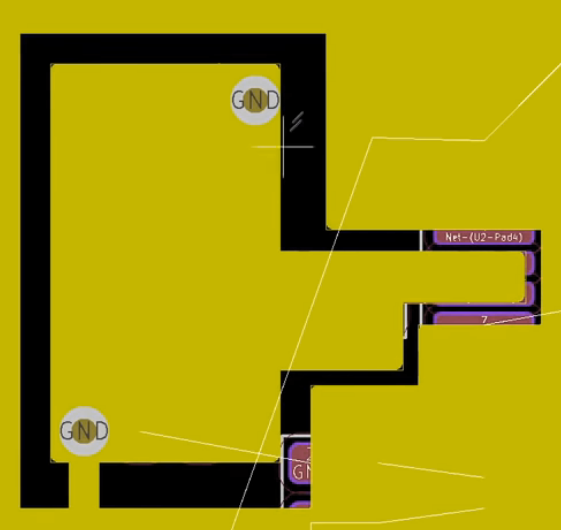
\includegraphics[width=\textwidth]{assets/isolated_gnd.png}
			\caption{Isolated ground plane should be connected to one point with the main ground, \href{https://www.youtube.com/watch?v=t5phi3nT8OU&t=4940s}{source}}
		\end{minipage}
		\hfill
		\begin{minipage}[b]{0.3\textwidth}
			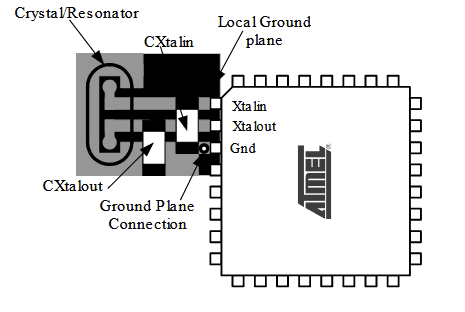
\includegraphics[width=\textwidth]{assets/layout_clock.png}
			\caption{\href{http://ww1.microchip.com/downloads/en/DeviceDoc/Atmel-8128-Best-Practices-for-the-PCB-Layout-of-Oscillators_ApplicationNote_AVR186.pdf}{source}}
		\end{minipage}
	\end{figure}
	
	\textbf{Question}: This discrete, isolated ground for the high speed signal of the clock traces can be used as a general technique for high speed signals?
	
	\subsubsection{Decoupling capacitors}
	
	% I will stick to the application note of TI, high speed layout guidelines. Decoupling is the same with bypassing
	Another huge factor that contributing to the power integrity of your design is the decoupling capacitors. It is worth mentioning that there are also the bypass capacitors and these terms are used interchangeably. So the decoupling/bypass capacitors are used to clean the power line from noise (low impedance path) and to provide a short burst of energy when the fast switching request power to drive the current. That's why for the decoupling, in order to cover a wider range of frequencies that needs to be shunt, we pick more than two capacitors. One for low frequency and one for high. Most of the times the vendors will provide the necessary information about the values. Or is this for the energy bursts? No I think
	
	%\href{https://electronics.stackexchange.com/questions/2272/what-is-a-decoupling-capacitor-and-how-do-i-know-if-i-need-one/2274}{resource}
	
	As we can see in the figure 22, if we didn't place a bypass capacitor, the urgent need of transistors for the charge to build up isn't satisfied by the power supply due to the inductance, the inertia of the power line. So we need to use a temporary power supply until the time that the system can reach the desired amount of current. 
	
	\begin{figure}[h!]
		\centering
		\begin{minipage}[b]{0.4\textwidth}
			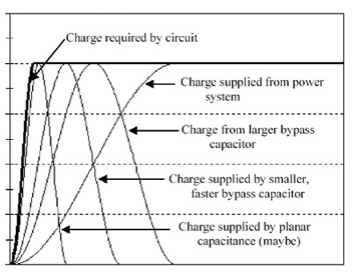
\includegraphics[keepaspectratio, width = \textwidth, height=.3\textheight]{assets/bypass_charge.png}
			\caption{Charge requirements of switching transistors, by Doug Brooks}	
		\end{minipage}
		\hfill
		\begin{minipage}[b]{0.4\textwidth}
			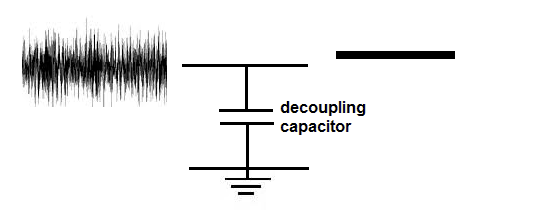
\includegraphics[keepaspectratio, width = \textwidth]{assets/decoupling.png}
			\caption{Smoothing the signal, \href{http://www.learningaboutelectronics.com/Articles/Decoupling-capacitor.php}{source}}
		\end{minipage}
	\end{figure}
	
	Another important thing for the decoupling capacitors is to place them \textbf{as close as possible} to the power supply pins of the component that you are trying to decouple. To minimize the inductance and to provide the energy as clean and fast as possible 
	%and to not let switching noise noise radiate, because they act as a low impedance path for noise as we mentioned.
	. If you have two capacitors with different values then place the smaller one closer. An interesting article for optimizing the decoupling capacitors location can be found here, \href{https://www.allaboutcircuits.com/technical-articles/pcb-layout-tips-and-tricks-how-to-optimize-your-decoupling-connection/}{all about circuits}
	
	
	
	\section{Parasitic elements}
	
	Not everything is what it seems! So far we said about the capacitance and the inductance of interconnections, but this also includes passive components, leads, connectors and so on. So it is quite important to be sure that you made the right choice of values for the passive components for the range of frequencies that you are interested along with proper PCB layout. Related to this frequency response is the so called self resonance, where for example capacitor acts like a complete pure resistor.
	
	\begin{figure}[h!]
		\centering
		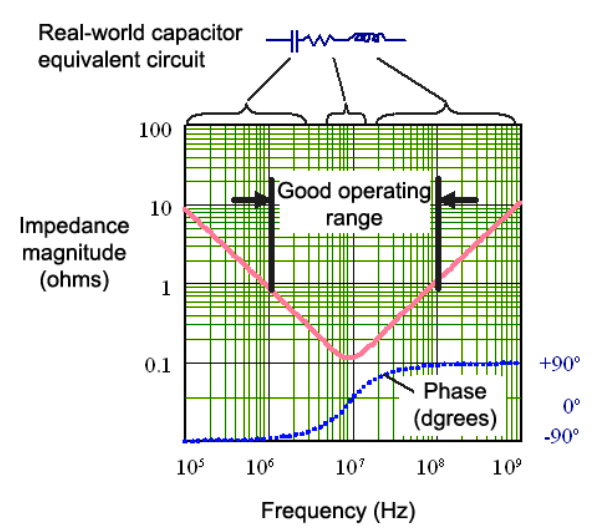
\includegraphics[keepaspectratio, height=.4\textheight, width = \textwidth]{assets/real_cap.png}
		\caption{\href{http://www.sigcon.com/Pubs/straight/resonance.htm}{source}}
	\end{figure}
	
	Most of the times we are referring to the magnitude of the impedance like high and low, but we are not mention anything about the phase. Should I care about phase? The digital circuit will work, but the analog components usually care about a lot about the phase so keep that in mind. Things change when frequency varies and remember in digital circuits we have a bandwidth and not a single frequency. (by \href{http://www.sigcon.com/Pubs/straight/resonance.htm}{source})
	
	\subsection{Component Placement}
	
	Before implementing any of those guidelines, the first thing that designers do is to place the component. Placement is referred as if not the most then one of the most important parts of the design. Some guidelines could be:
	
	\begin{itemize}
		\item Give room to breathe! Consider the density of the traces that will run across the board.
		\item Partition the design (RF, digital, analog). Group similar parts together.
		\item Connectors should be placed to the edge of the board away from circuitry.
		
		Input/Output pins is a very common way for noise to be coupled on and off the board. So for this reason should be placed away from the rest of the circuitry, in the edge of the board, source: A brief annotated list PCB EMC Design Guidelines
		
		\item Components that are \textbf{thermal} critical should not concentrated in a the same area in order to avoid hot spots. So distribute them and don't place them near the edge, because the heat removal won't be the best. \href{https://www.allaboutcircuits.com/technical-articles/pcb-thermal-management-techniques/}{source}
		
		\item Decoupling caps as close as possible to power and ground pins.
		\item Check the \textbf{ratsnest}\footnote{Ratsnest is a bunch of air wire connections that show the distance of the connections in the PCB layout} and find the most efficient way for the traces to be short and with less via.
		\item Design for assembly. It is generally preferred to have the IC the same orientation but it isn't mandatory.
		\item Sometimes rotating the IC with an angle of 45 angle can help in the next steps of routing.
		\item Don't forget the mechanical dimensions. Components should not overlap.
	\end{itemize}
	
	Finally an objective/artistic comment is that if it looks good it will work!
	
	\subsection{Routing}
	
	How to connect something? Let's have an overview of the different ways of routing. \href{https://resources.pcb.cadence.com/blog/pcb-routing-topologies-demystified}{source} Namely we have:
	
	\begin{itemize}
		\item Daisy chain
		\item Point to point
		\item Star connection
		\item Bus
	\end{itemize}
	
	\subsection{Mixed design}
	
	%Guidelines for designs that include analog, digital and RF signals. Partitioning, but what this actually means?
	
	How to approach design including analog, digital or RF components? Should I split the ground? Be aware the return paths, the slots and not to overlap currents from different functional groups.
	
	
	%As the frequency gets higher the impedance is dominated by reactance and not resistance. But when this happen? We will propably find out. I mean everything has inductance and capacitance and they are function of the length and the frequency. So what is the equivalent rule of thumb? Like the transmission problem? Maybe there isn't because a lot of factors contributing to these. But let's see how eric bogatin measure the capacitance and inductance. Inductance and capacitance is for sure a function of the frequency. The reactance of the traces is inherent but it shows only when high frequency.
	
	\subsection{Mounting holes}
	
	%Do your remember the era and how much time you are devoted to demystify for the clearance, vias on the holes and so on? For the EM report that was as I can recall.
	
	%But let me tell you my pain. The most important thing that needs to be addressed is design for performance and simulation aspect of PCB that we actually skipped in the PCB thing but I trust you that you can do stuff. You have 5 more days to do only Acubesat work. 5 August it is a necessity to working for uni and divide your time into Acubesat and uni until 15 August. Then we have only uni things. OKay, I think it is doable!
	
	Why there is clearance on the mounting holes? Should I ground them? Should I put vias on them?
	
	\begin{figure}[h!]
		\centering
		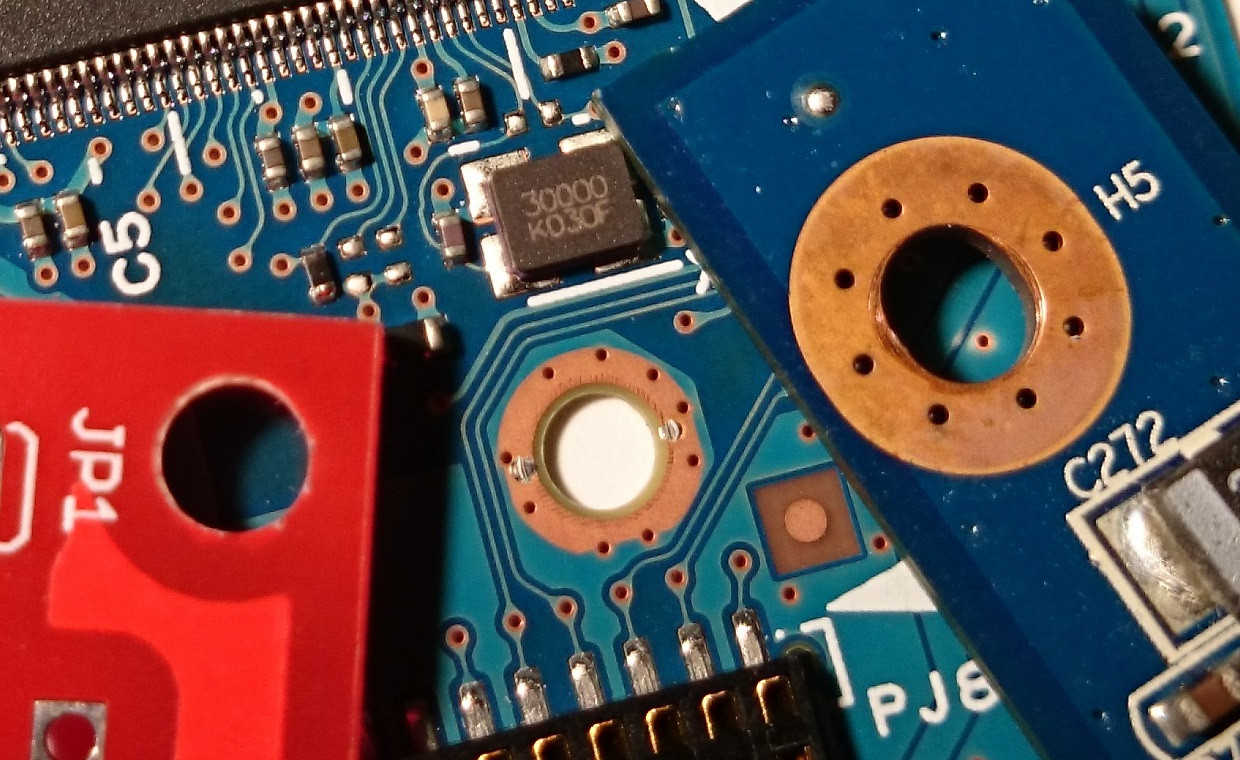
\includegraphics[keepaspectratio, height=.3\textheight, width = \textwidth]{assets/mounting_holes.jpg}
		\caption{Different types of mounting holes \href{https://atadiat.com/en/e-four-pcb-marks/}{source}}
	\end{figure}
	
	%\subsection{Decoupling capacitors}
	
	%How to place the decoupling capacitors, via vs trace, inductance of plane, inductance of via and small tracks. Check this article . This may be an overkill for our design. Vias should be used when having planes, but not for intersecting the layers due to EMI, place ground transition vias though. What is the arguement for using not many vias? Ground loop, no. Cost in the manufacturing? Impedance matching? Breaking the planes if they are through hole vias?
	
	%Decoupling vs bypass. Smoothen vs shunt the noise. 2 caps for decoupling indicate by datasheets. The voltage drop thing is for the current carrying the plates that can de-charge the capacitor and have voltage drop, thus higher capacitance the better. How to increase the capacitance? Spreading caps all over?
	
	%Interesting articles for decoupling: \href{http://www.sigcon.com/Pubs/straight/resonance.htm}{1}, \href{https://resources.altium.com/p/should-you-use-your-power-plane-as-a-return-path}{2}, \href{https://electronics.stackexchange.com/questions/274346/bypassing-vs-decoupling-capacitors}{3}, \href{https://components101.com/articles/decoupling-capacitor-vs-bypass-capacitors-working-and-applications}{4}
	
	\subsection{Unused pins}
	
	Most of the times the datasheets will provide information what the designer should do about the unused pins, the floating pins of an MCU for example. The common solution is to tied them to ground, providing a low impedance path. But is this always the case? Is a myth to tie every floating pin to ground (\href{https://learnemc.com/not-so-good-emc-design-guidelines}{food for thought})?
	
	%\subsection{2 Layer design}
	
	%2 layer design is a special and very common in PCB. Some specific tips for this type of design are the following:
	
	%\begin{itemize}
	%	\item Horizontal traces above, vertical below.
	%	\item Use the leftover area, make it ground
	%	\item Be careful with slots. This is a general rule of thumb though
	%\end{itemize}
	
	
	\section{Design for Manufacturing}
	
	In order for the PCB to transition from the Gerber state to reality, it should be manufacture-able! Therefore DFM (Design for Manufacturing) guidelines should be taken into account early at the design stage\footnote{The design stage is the most cost efficient stage to detect and fix potential problems} to avoid product failures and save time and money. 
	
	Even if something can be fabricated, small changes in the layout can reduce the total cost. This isn't always the case for small quantities but at mass production scale, even the smallest nuances will increase it significantly. 
	%\href{https://resources.pcb.cadence.com/blog/2019-product-development-for-electronics-and-hardware-planning-for-scaling}{source}. 
	
	Usually EDA tools feature \textbf{DRC} (Design Rule Checking) tools, that automatically inspect the board to determine whether it meets the constraints imposed by the manufacturer.
	%(for compliance with standards used by the manufacturer)
	For instance, Eurocircuits offers some \href{https://www.eurocircuits.com/drc-settings-and-guide-lines-for-cad-packages/}{templates} to import these scripts to the EDA tool used by the designers (for this case the supported ones are KiCad, Altium and Eagle). It should be noted that DRC is usually checking for trace width, spacing and enclosure, but this is only a subset of the DFM. So it is quite important to have an overview of the methods that are going to be used for the fabrication of the PCB. DFM is sometimes referred not only to the bare board production but also to the assembly (Design for Assembly). Actually, DFM and DFA automatic checks are the first things that the manufacturers do. 
	
	It is recommended to know in the design phase how your PCB will be assembled to integrate the corresponding considerations and rules. Some guidelines for DFM outside the scope of DRC could be:
	
	\begin{itemize}
		\item All component outlines on your silkscreen should be marked with a reference designator and polarity (pin 1 marker) indicators. 
		
		About polarity, there is also the option to export a dedicated layer for this purpose from your EDA tool (Fab layer for KiCad) as we have already mentioned.
		% \href{https://www.altium.com/design-manufacturing-resources}{Altium source DFM}
		
		% \href{https://www.seeedstudio.com/blog/2019/06/12/how-to-generate-assembly-files-and-why-they-are-important/}{source for assembly data}
		
		%\item Placing and orienting components
		\item Prefer to place all the components to the top side of the board. Double sided PCBs are costly. If component placement is done with automatic pick and place machines, then additional cycle is required in the assembly line to flip the board and do the placement on the bottom side.
		\item Orient similar components in the same direction. It is easier for inspection and testing. It looks nicer too!		\item How my PCB is going to be assembled/soldered? Manually or by automated machinery? Reflow or wave soldering?
		
		If \textbf{wave soldering} is going to be used then for optimal soldering the designer should consider: 1) The SMDs are aligned perpendicular to the direction of the board going through the wave, 2) Large components should not "shadow" smaller ones and 3) Dual in line packages such as SOIC have their axis aligned to the wave direction. 
		
		%\href{https://www.vse.com/blog/2020/01/21/component-orientation-on-pcbs-best-practices-to-optimize-assembly/}{source}
		
		In general the assembly house could provide some guidelines analogous to the soldering method. 
		
		%Some packages may can't wave soldered properly like QFP, because leads are located in all sides and trailing pins should be shadowed.
		
		%Place the two pictures by the eagle autodesk. How to place two figures side by side? The bad and good
		
		\begin{figure}[h!]
			\centering
			\begin{minipage}[b]{0.4\textwidth}
				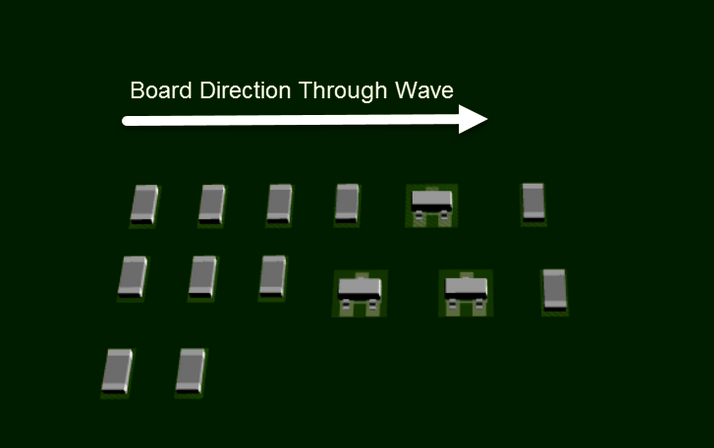
\includegraphics[width=\textwidth]{assets/good_wave.png}
				\caption{Good orientation for wave soldering,\href{https://www.autodesk.com/products/eagle/blog/top-10-pcb-component-placement-tips-pcb-beginner/}{eagle}} 
			\end{minipage}
			\hfill
			\begin{minipage}[b]{0.4\textwidth}
				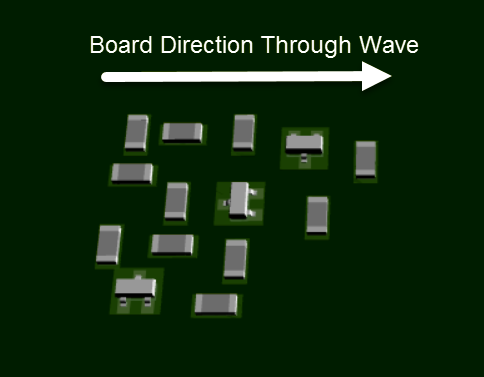
\includegraphics[width=\textwidth]{assets/bad_wave.png}
				\caption{Bad orientation for wave soldering}
			\end{minipage}
		\end{figure}
		
		For manual assembly, consistency in the component placement can aid a lot the assemblers and make the process less error prone. For example it would be helpful if all ICs is oriented so the pin 1 is located in the same direction.
		% (source, the Orcad book in the DFM section)
		
		\item Although placing via on pads is great in high speed application, assemblers tend to recommend not doing that because solder can wick into the hole thus a poor joint is created.
		
		%\href{https://macrofab.com/blog/via-in-pad-pcb-design/}{source}
		
		\item Place 2 or 3 fiducial (reference points for the pick and place machine) marks, which should not be covered with the solder mask. Generally, these should be placed diagonally in the corners of the PCB. The pick and place machine finds these points using a camera and all components are placed on the coordinates relative to these points (tip: The bottom left corner of the PCB outline should be selected as the origin (0,0) point). 
		
		%\href{https://uk.beta-layout.com/pcb/technology/assembly_guide.html}{source}
		
	\end{itemize}
	
	It is worthy mentioning that some times \textbf{conflicts} emerge when trying to design for manufacturing and performance (functionality) at the same time. Some DFM rules may violate DFP ones and the opposite, that could increase the manufacturing cost. So a \textbf{trade-off} mindset is very common! It is also important to contact the assembly house to understand and identify the requirements of the DFM.
	%For example double sided boards, or placing vias all over the place, vias on pads (some parts may not solder properly), routing topology and orientation.
	
	Footprint design is also related with DFM. In order to meet manufacturing (soldering, stencil and soldermask) requirements and electric performance criteria, pad size for each layer (copper, stencil, soldermask) should be designed in a suitable manner. For this purpose footrpints are usually compliant with industry standards like IPC-7351.
	
	\section{Testing}
	
	The PCB development cycle is consisted by 4 main parts: 1) component selection and design layout, 2) manufacturing, 3) assembly\footnote{Fabrication and manufacturing sometimes can be referred to the bare board production and the assembly or only to the first one} and 4) testing. Testing is integrated both in the manufacturing and the assembly.
	
	Each manufacturer for the bare board production is following certain guidelines to ensure and control the quality of the board. These are based on industrial standards. For example, Eurocircuits is compliant with the IPC-A-600 Class 2, the most used one in the industry. In summary, this manufacturer combine  automatic optical inspection, flying probe testing (doesn't need test fixture) and human inspection. \href{https://www.eurocircuits.com/making-a-pcb-pcb-manufacture-step-by-step/}{source}. A more detailed approach for the Eurocircuit's inspection workflow can be found here  \href{https://www.eurocircuits.com/blog/how-do-we-assure-the-quality-of-your-pcb-part-1/}{source the 3 parts blog}
	
	Once the board is fabricated, the next step is the assembly process (PCBA). The assembly house is responsible to populate the bare board with components and to detect and fix the defects (mention defects like what?) along the way. Methods used to spot defects are typically:
	\begin{itemize}
		\item Automatic optical inspection (AOI).
		\item X-Ray inspection, also called AXI.
		\item Flying probe testing. Probes moving around the board trying to contact the test points and components.
		\item JTAG Boundary Scan. Actually JTAG isn't used only for programming and debugging MCUs, but it was created initially for assembly testing.
		\item Functional testing. 
	\end{itemize} 
	
	\begin{figure}[h!]
		\centering
		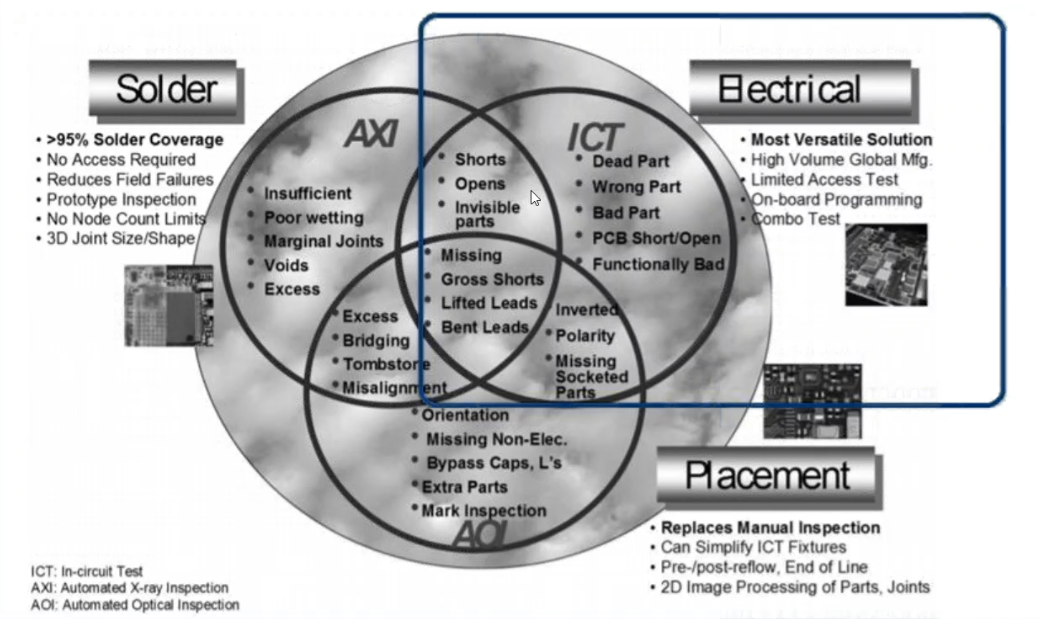
\includegraphics[keepaspectratio, width = \textwidth, height=.4\textheight]{assets/testing_overview.png}
		\caption{Testing overview by SMTA/TMAG TP-101E standard}
	\end{figure}
	
	But there is also a number of defects that can't be spotted by visual inspection (accessibility limitations), so a more complex testing method along with design requirements (test fixtures) is coming to the surface. 
	
	This method is called in-circuit testing (\textbf{ICT} aka bed of nails) and can ensure that the board can move in the production line with zero defects. These defects include solder bridges, shorts, opens, resistance, capacitance, missed components etc. In short a group of probes are interfacing with usually one side of the PCB  by placing test points\footnote{Test point: A small exposed copper area used as a connection point to test circuitry on a PCBA} to all the nets. For this to happen, a test fixture is required that increases significantly the cost.
	
	%\href{https://www.altium.com/solution/designing-for-testability-pcb-design}{source}
	
	\begin{figure}[h!]
		\centering
		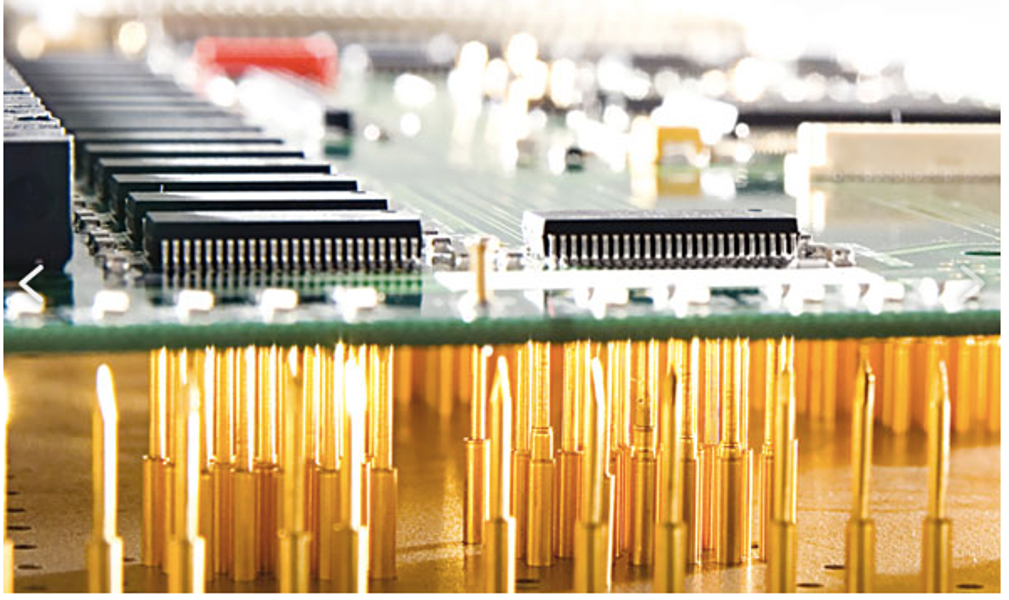
\includegraphics[keepaspectratio, width=\textwidth, height=.25\textheight]{assets/bed_of_nails.png}
		\caption{A bed of nails test fixture \href{https://hackaday.com/2019/02/09/test-pcbs-on-a-bed-of-nails/}{source}}
	\end{figure}
	
	%E.g. it is also possible to boot the board to some bootloader and execute tests available in the bootloader, test Ethernet connections, test USB connections, ... No need to say that this comes at a cost.\href{http://www.nod-pcba.com/pcb-assembly-process/pcb-assembly-testing-methods-en.html}{source}
	%For the last one, in circuit testing (is used also for simple defects like open, shorts etc.) and flying probes are the most known ways to address it. 
	Assemblers charge the customer by the type of the testing service and by the hours needed which is a function of volume. In general testing is an expensive part of the cycle.
	% (, typically the 30\% of the total cost. \href{https://www.altium.com/solution/designing-for-testability-pcb-design}{source about the cost}).
	The cost for ICT is on average 20.000 dollars! 
	%Another resource for the cost, \href{https://en.wikipedia.org/wiki/Flying_probe}{wiki} and \href{https://blog.matric.com/what-does-pcb-in-circuit-testing-cost}{source}. 
	Testing for electric performance (verify proper operation for analog and digital circuits) could also be integrated in the provided services as part of the ICT by performing power up tests. It can test for functionality as well as assembly defects.
	
	On the other hand, bed of nails technique has \textbf{limitations}. For example in packages like BGAs and in high density boards, placing test points is very inconvenient. So JTAG interface comes for the rescue and aids the assemblers for the testing process. Requirement for JTAG boundary scan is the device under test to have a built in controller or to be accessed implicitly by another device capable for JTAG interface (e.g. Testing a memory module via an MCU with built in JTAG).
	
	% source for the jtag info is the eevblog guy, video what is jtag?
	
	%\href{https://www.acceleratedassemblies.com/blog/in-circuit-testing-the-best-technique-to-detect-manufacturing-faults/}{source}
	
	%The are several inspection methods, including hands-on inspection by a person, automatic optical inspection that relies on image recognition, and even x-ray inspection to look through components that may block an inspector’s view. \href{https://telancorp.com/pcb-assembly-process}{source}
	
	%Πρέπει να σημειωθεί ότι δεν μπορούμε να καλύψουμε οτιδήποτε γύρω απο τον κόσμο του PCB design, προσπαθούμε κάπως να δώσουμε ένα ερέθισμα, μια τροφή για σκέψη...
	
	Finally there is the \textbf{functional testing} (FCT). Its purpose is to simulate the environment in which a product is expected to operate (Does everything work together?). Functional testers typically use a computer that is connected to test points or a test-probe point in order to perform FCT.
	%(For that purpose a range of different signals are applied to check the electric behavior of the board and to determine)
	It can check if all external analogue and digital inputs and outputs meet the requirements and the specifications. Functional testing can use the JTAG or the test fixture for the interface. 
	
	%\href{https://www.pcbway.com/pcb_prototype/PCB_Assembly_Functional_Testing.html}{source}
	
	%source about the interface is the fact that test fixture act as a funnctional interface too and from the EEVBlog talking about JTAG
	
	Does it \textbf{worth} to include test fixture and the additional \textbf{cost}? In circuit testing and flying probe testing is a quite common debate. In general for low volume, prototypes and low complexity boards, flying probe testing is the way to go along with visual inspection and functional testing. Flying probe testing is referred also as a type of in-circuit testing but without the need of the "bed of nails", the test fixture. The drawbacks are: more cycle time, less test coverage (how to test BGA with flying probes?), no power up test etc. But usually a combination of methods can also be used. 
	
	% resource that combinations of methods can be used, \href{https://en.wikipedia.org/wiki/Flying_probe}{source}
	
	A good resource about flying probe testing, \href{https://blog.matric.com/flying-probe-test-capabilities}{capabilities of flying probe testing}
	
	%Along with most other tests, flying probe testing does not power up the circuit. So you don't get the true real-world look at your product the way an ICT gives you, \href{https://blog.matric.com/flying-probe-test-capabilities}{source}
	
	%\href{https://www.vse.com/blog/2019/10/01/understanding-in-circuit-test-vs-flying-probe-for-your-pcba/}{source}
	
	% more about ict vs flying, \href{https://blog.matric.com/ict-testing-vs-flying-probe-testing}{source}
	
	%NICE: The advantages of ICT are that it can test for functionality as well as for assembly defects, \href{https://www.vse.com/blog/2019/10/01/understanding-in-circuit-test-vs-flying-probe-for-your-pcba/}{source}. I think the same applies for the JTAG
	
	\subsection{Design for Testing}
	
	%Each type of testing that the assembly house can provide, has some requirements that need to be addressed in the design stage. These can be for example the location and the type (size and shape) of the test points.
	
	%As we have seen the list of the possible tests that an assembly house can provide, the design requirements for each kind of testing should be mentioned.
	
	Among the first things that the designer should definitely ask is how the board is going to be tested (planning ahead is crucial). There are quite a few rules that need to be addressed for testing, especially for ICT and flying probe testing. Some of them could be:
	
	\begin{itemize}
		\item Place test points to each net being accessible from the bottom or the top of the PCBA. Preferably, to minimize the cost, use only one side (no need for an extra cycle in the assembly line) 
		
		%\href{https://www.jjsmanufacturing.com/blog/9-pcb-assembly-design-guidelines-for-flying-probe-test}{source for flying probe testing}. For ICT it is strictly from the bottom? I think no
		
		\item Distribute test points evenly over PCB. Don't have too many test points in the same area. 
		\item Design the shape and size of test points according to the probes that are going to be used by the assembler.
	\end{itemize}
	
	A standard recommended for testability guidelines is the "SMTA/TMAG Testability Guidelines TP-101E".
	%In large volume production testing (functional, electric performance) is integrated in the assembly stage. But testing for functionality and electric performance can be done also by the user. So the test points should be configured in a way to be compliant with the probes of the electric instruments that are going to be used to analyze the electric signals. The designer obviously should determine which signals should be analyzed and place the test points accordingly. It is worth mentioning that placing more than one test points for the power supply in different areas of the board is also a good trick to inspect the integrity of the power and the ground.
	
	Functional and electric performance testing can also be made manually. In this case, similar with the above guidelines for the automatic testing, the designer should place the test points to the nets of interest being \textbf{accessible} from the top or the bottom. The electrical instruments that are going to be used should also be considered to adjust the \textbf{shape} of the test points with the probes. Prob tips can help to clip the test points without using hands to handle them. Sometimes for \textbf{practical issues}, using vias uncovered with solder mask, can make using electrical instruments more easier than just a flat pad surface. In high speed signals, getting an accurate view of the tested signal via contacting probes to test points can be quite challenging. Thus the electrical characteristics of the probes should be considered. For example, to minimize the inductance of a long ground lead, provide a ground point near the measurement of the signal to make the loop smaller for signal integrity. Finally, place test points everywhere, the more the merrier, but be mindful regarding the following statement. 
	
	% source about minimize the loop for the probes, \href{https://www.eevblog.com/forum/eda/test-points-for-mediumhigh-speed-signals/}{source}
	
	% Fun question: When probing, it is like stealing the signal from the circuit and isolate a specific track from the rest? I mean the signal isnt divided to circuit and oscilloscope? If I provide a low impedance path then the signal will go to the oscillloscope right? and not to the rest of the circuit? If I have a led for example, will it produce light, if I probe the signal with very low impedance?
	
	%\textbf{Should I take into account the impedance matching with the probe and the signal of interest, test point?}. . To mitigate reflections and attenuation should the designer consider the impedance of the probe and of the test point?
	
	% source for probe impedance and tet point:\href{http://www.sigcon.com/Pubs/news/3_2.htm}{this}
	
	% manual testing, via vs pad, \href{https://electronics.stackexchange.com/questions/48557/testpoints-vias-versus-pads}{source}
	
	% \href{https://starfishmedical.com/blog/pcb-design-tips/}{more info about test points for the manual part}
	
	%You can add something like a life hack: Clipper for probe for the test point.
	
	%A nice question for manually testing, \href{https://electronics.stackexchange.com/questions/308025/how-to-create-measurement-points-on-a-pcb-for-diagnostics/308032}{this}
	
	% about probing tip, \href{https://electronics.stackexchange.com/questions/480846/what-probe-tip-to-use-to-clip-into-a-pcb-test-point}{source}
	
	
	As we have already mentioned in the DFM, in a similar way the DFT can emerge conflicts with the design for performance (DFP). Creating holes to each net in a tight space isn't always an easy thing to do and in high speed applications, test points can cause performance issues. Some traces due to the above reasons might not be tested at all. Thus design for testing might have some drawbacks but it can save a lot of cost in the long run. 
	
	%courtesy of EMA-EDA webinar DFT, what designer need to know about testing \href{https://pages.ema-eda.com/EMA-2020-Webinar-Desiging-for-Test}{source}
	
	%\textbf{Resources} for the above is for sure the webinar EMA we have watched! And a lot of assembly house documentation and blog post. I dont think that you can find relevant literature resource for this. Only some kind og generic books like the Hitchikker guide and the orcad design book.
	
	
	
	\section{Simulation and analysis}
	
	Simulations can be thought as a method to predict the future that can save a lot of time and cost in the long run. Imagine to be able to know that your board is functional and meets the specifications only if it was manufactured. Then it would take probably ages to finalize the design. So the intermediate way to increase the confidence of the design is achieved by creating a virtual representation of the product's behavior. The virtual world is now our playground without worrying about the cost or the risk of failure. Basically, engineers are trying to catch up with potential issues that could eventually arise when the design becomes a real piece of hardware.
	
	%By integrating them in the development cycle, engineers are trying to catch up with potential issues that could eventually arise when the design becomes a real piece of hardware. For practical reasons (less computational time and resources) it is recommended to simulate critical traces like clock or other high speed signals. 
	
	Creating a virtual world that is identical with the physical one is quite a challenge. Thus for practical reasons (less computational time and resources) it is recommended to simulate only critical traces like clock or other high speed signals.
	
	The simulation can be divided into three main groups: 
	
	\begin{itemize}
		\item Simulate the \textbf{circuit model}, a translation of the board layout. 
		%(Consider the distributed model though. But schematic is a group of lumped elements related with each other.)
		Don't forget the distributed model and consider the interconnections as transmission lines.
		
		SPICE related tools for this type of modeling that are used in the industry are LTSpice, PSpice, Multisim, Proteus and the \textbf{QUCS} (open source). Also most of the EDA tools provide built in circuit analysis based on SPICE models. KiCad can support circuit simulation and is based on the \href{http://ngspice.sourceforge.net/ngspice-eeschema.html}{ngspice} engine.
		
		
		\item \textbf{Electromagnetic} analysis with \textbf{S-parameters} and a corresponding simulation tool. The S parameters can be obtained either using an electromagnetic simulator having as input a compatible version of the physical layout or can be measured directly using electrical instruments such as vector-network analyzer. 
		
		Some tools to simulate Maxwell's equations are: Ansoft’s High-Frequency Structure Simulator (HFSS), Clarity 3D Solver by Cadence, CST PCB STUDIO and some open source ones like \href{https://www.opensourceimaging.org/project/open-ems-a-free-and-open-electromagnetic-field-solver/}{openEMS} and \href{https://www.fastfieldsolvers.com/}{Fast Field Solvers}.
		%But when to use such tools? When you don't have uniform lines (discontinuities), like vias, packages, connectors and the designer wants to have an overview of the electromagnetic phenomena for these cases.
		Numerical solution tools like Matlab, Octave can be used for modeling with S-parameters too.
		
		\item Specialized \textbf{signal integrity simulators} like HyperLynx and Cadence.
		% A \href{https://www.signalintegrityjournal.com/articles/199-useful-sipi-tools-from-istvan-novak}{list} of useful tools. \href{http://www.sigcon.com/Pubs/straight/planningsi.htm}{source}
		
		These commercial tools have many benefits than the traditional circuit simulators. They can import a trace layout and perform a lot of automatic checks to find and solve problems about signal integrity. They use the IBIS model (we will mention it later).
	\end{itemize}
	
	\subsection{Circuit vs EM simulation tools}
	
	Neither of these tools individually is enough to have a complete representation of the circuitry and to identify the SI, PI, EMC problems. EM field simulators can handle EMC problems, resonance and non uniform wave propagation and considerations regarding the trace geometry such as how bad is this slot in a specific return path. The circuit simulator can handle switching noise (ground bounce), near field crosstalk, transmission line propagation and reflections.	
	
	PCB design is a very complex structure. Usually tools that solve 3D Maxwell equations can handle simple ones and require expertise and a very good understanding of electromagnetism. So the circuit simulation, if you need to choose between these two, in most cases is preferable. It is quicker and easier to use and can offer an adequate representation of the physical layout.
	
	\subsection{Circuit modeling}
	
	A very good \href{http://www.sigcon.com/Pubs/straight/planningsi.htm}{resource} by Howard Johnson for overview about simulation.
	
	What is modeling? "Modeling refers to creating an electrical representation of a device or component that a simulator can interpret and use to predict voltage and current waveforms". The devices can be divided to the active (e.g. transistors) and the passive (e.g. interconnections)ones. For the first, there are two types of models, the SPICE and the IBIS.
	
	The SPICE model is well known in the world of circuit simulation and is used in the analog simulation tools based on the SPICE engine. However, vendors usually struggling to offer these type of models for their products because precious information can be obtained regarding the design of the IC. Thus without revealing the intellectual property of the product, vendors usually provide the so called Input/output Buffer Information Specification (\textbf{IBIS}) model that run in special signal integrity simulators (or behavioral simulators) of the industry, like the ones mentioned before, while containing only the necessary data for this type of analysis. Simulations tools that can handle these models are mostly commercial and probably the most complete tool among them is the HyperLynx provided by Mentor.
	%Can you view the IBIS model to contain valuable data about the rise time of signals though? Or something useful to determine how critical they are?
	However, IBIS models can be useful, even without simulation, by \textbf{viewing} their data that contains among others the rise time of signals in the digital ports.
	
	An extensive resource to IBIS models is \href{https://www.analog.com/media/en/technical-documentation/application-notes/AN-715.pdf}{this by Analog}. Nice wording too.
	
	%It is worth mentioning that in digital circuits with complex devices like MCUs, there is no point creating a SPICE model for them. It is more convenient to simulate specific digital ports of interest. A simple simulation could include in the schematic capture a driver, a load and the interconnection, the transmission line with impedance set by the PCB layout. 
	%(Its impedance is a function of the width and the thickness and can be calculated using online tools such as the Samacsys or integrated tools of the EDA tool)
	
	These traditional \textbf{analog} tools, based on SPICE, can do the work for the common digital scenarios. The question is how to build or find spice circuit models for the transmitter and the receiver? How to approximate the circuit, how to test and model high speed signals? How to integrate the inductive and capacitance coupling to your circuit? Can 2D and 3D fields results interpreted as lumped elements and included in my simulation (because crosstalk can't be seen by a schematic, but affects the design)? Circuit modeling using SPICE models should be a topic for a new report!
	
	
	%\subsubsection{Workflow}
	%\textbf{First route the critical traces}
	
	\section{Rules of thumb}
	\label{subsec:thumb}
	
	\begin{itemize}
		\item In general keep traces short and wide
		\item Keep signals and their return paths as close as possible. Avoid slots in planes or keep them short
		\item Be aware of the return current paths and try to visualize how current will flow (easy to say, hard to do!)
		\item Spread unrelated signals as further apart as possible and keep the distance, that these signals are adjacent, short
		\item Slow down the signals (clock frequency) if there is no need of higher frequencies
		\item Provide low-impedance path for the power supply and ground
		%\item Be aware of the sources of EMI and victim. Eliminate the interference and protect the victims!
		\item Identify the vulnerable parts of your PCB design and partition it efficiently. What components are sensitive in power-supply terms? What is the rise time of this data signal? What should I do when mixing analog and digital signals? What precautions should I take?
		\item Impedance control and termination if it is required
		\item Decoupling caps!
		\items Read the datasheets to find any specific required hardware support
		\item Don't forget the manufacturing process and design accordingly to the manufacturer (e.g. orientation of components)
		\item Unused pins should be tied to the ground
		\item Avoid ground loops
		\item Use vias with care
		\item First route the critical traces
		\item An old saying is that PCB design is 90\% placement and 10\% routing.
		\item PCB is art! If it looks good, it will work good!
	\end{itemize}
	
	\section{Checklist}
	
	\begin{itemize}
		\item Did you read the datasheets and the docs in general for the hardware development of each component offered by the vendors?
		\item Did you place decoupling capacitors?
		\item Did you know the logic family, the voltages, the current, the rise time? How critical is your design?
		\item Do I need to take into account reflections? 
		\item RF, Digital, Analog?
		\item Are you sure that everything fits? Mechanical constraints?
		\item Did you run the DRC check?
		\item What are the tolerances, the noise margins? 
		\item What was the trade offs between cost and functionality to meet the requirements?
		\item Did you design for manufacturing and testing? Who is gonna do the testing?
		\item Did you make simulation to increase the confidence for the functionality of your board? 
		\item Are the assembly and manufacturing data with the proper format and compliant with the needs of the corresponding house?
		\item Are you sure that ground is ground?
		\item Are passive components like capacitors and inductors what they are supposed to be? Parasitic elements?
		\item Do you like the aesthetic aspect of your PCB (PCB is art!)? If yes then you are probably going well.
		\item Do you plan to improve this checklist? (It would be wise to do so!)
	\end{itemize}
	
	\section{Endnote}
	
	Along the way we have mentioned a lot of rules of thumbs but we didn't mention the most important one. Don't take rule of thumbs too seriously. These are approximations and sometimes can differ a lot from reality. If designer want to think something fast then it is an okey method. But simulations along with specific data for your application is a more accurate but time consuming process. 
	
	Warning, a biased opinion is following: If Balanis book is the bible for Antenna theory then Signal Integrity and Power Integrity by Eric Bogatin is the bible for PCB design.
	
	
	
	\section{Resources}
	\subsection{Learning resources}
	\begin{itemize}
		\item[-] Howard Johnson, Martin Graham. High Speed Digital Design: A Handbook of Black Magic 
		\item[-] Peter Wilson. The Circuit Designer's Companion
		\item[-] Mark I. Montrose. Printed Circuit Board Design Techniques for EMC Compliance 
		\item[-] Douglas Brooks. Signal Integrity Issues and Printed Circuit Board Design
		\item[-] \href{https://drive.google.com/file/d/1C4cFAzJpTlKedcgKvlWDQnTaCCgdo58s/view?usp=sharing}{EMC Fastpass. Getting EMC design right at the first time}
		\item[-] \href{https://drive.google.com/file/d/1mr8UNMDeXmdCBnOVq22b1YUi3WwKNUMm/view?usp=sharing}{Texas Instruments. High-Speed Layout Guidelines}
		\item[-] \href{    https://drive.google.com/file/d/1gwrVG8WULKCOxYYrVLvCCZh1-luvQacq/view?usp=sharing}{NXP. High-Speed Layout Guidelines}
		\item[-] \href{https://drive.google.com/file/d/1ylptbGbczsr2scbjPCba7q4J1PiyvQL8/view?usp=sharing}{David L. Jones. PCB Design Tutorial}
		
	\end{itemize}
	
	\subsection{Notorious websites}
	\begin{itemize}
		\item \href{https://bethesignal.com/bogatin/}{Be the signal}
		\item \href{http://www.sigcon.com/}{Howard johnson}
		\item \href{https://www.signalintegrityjournal.com/}{Singal integrity journal}
		\item \href{https://www.edn.com/}{edn}
		\item \href{https://www.allaboutcircuits.com/}{all about circuits}
		\item \href{https://incompliancemag.com/topics/resources/}{incompliance magazine}
		\item \href{https://electronics.stackexchange.com/questions/15135/decoupling-caps-pcb-layout/15143#15143}{An amazing stackexchange answer. Definitely worthy to give it a read!}
		\item \href{http://www.hottconsultants.com/}{Henry Ott}
		\item \href{https://learnemc.com/}{LearnEMC}
	\end{itemize}
	
\end{document}